\chapter{Parts i construccions universals}\label{cap:parts}

\begin{objectius}
\apartat{Prerequisits} El capítol~\ref{cap:aplicacions} complet: el llenguatge formal i els convenis de notació, la composició i les lleis de neutralitat, els elements generalitzats i el criteri d'igualtat, els isomorfismes, el conjunt terminal i l'inicial, i l'axioma de separació global, que aquí només s'usa a les observacions de lectura clàssica. De la teoria clàssica de conjunts, n'hi ha prou amb la familiaritat informal amb subconjunts, funcions característiques, unions disjuntes i productes cartesians, que es reconstrueixen al capítol.
\apartat{Objectius} En acabar el capítol, el lector hauria de poder:
\begin{itemize}
  \item definir monomorfisme i epimorfisme per cancel·lació, i demostrar-ne les propietats bàsiques: identitats, composicions, isomorfismes, seccions i retraccions;
  \item explicar per què una part d'un conjunt és un monomorfisme, i no un conjunt, i treballar amb la inclusió i la pertinença generalitzada com a factoritzacions;
  \item reconèixer quan dues parts són equivalents i com recuperen, en el metallenguatge, la noció de subconjunt;
  \item enunciar la propietat universal d'una suma i d'un producte, escriure l'aplicació definida per casos i l'aparellament, i demostrar la unicitat llevat d'un únic isomorfisme;
  \item usar l'axioma de representació: associar a cada part la seva característica cap a \(\mathbf2\), i deduir-ne que els bimorfismes són isomorfismes;
  \item construir equalitzadors i pullbacks a partir dels productes i de la representació, sense cap axioma nou, i deduir-ne la imatge inversa i la intersecció de parts;
  \item situar la injectivitat, l'exhaustivitat i la bijectivitat clàssiques respecte dels monomorfismes, els epimorfismes i els isomorfismes, i saber quines equivalències depenen de la separació global.
\end{itemize}
\end{objectius}

Al \hyperref[cap:aplicacions]{capítol anterior} hem fixat el llenguatge de la teoria i hem introduït les nocions d'aplicació, conjunt, composició, isomorfisme, conjunt terminal i conjunt inicial. També hem establert els convenis de notació i la representació geomètrica del metallenguatge mitjançant diagrames d'aplicacions. En aquest capítol començarem a construir nous conjunts a partir d'altres conjunts.

El principi que guiarà totes les construccions serà el mateix. No descriurem un conjunt nou indicant de quins elements globals està format, sinó especificant les aplicacions que hi arriben o que en surten i les equacions que aquestes aplicacions han de satisfer. Les propietats que caracteritzen d'aquesta manera una construcció s'anomenen \emph{propietats universals}.

Abans d'introduir-les, necessitem dues classes d'aplicacions definides exclusivament mitjançant la composició: els monomorfismes i els epimorfismes. Els monomorfismes ens permetran definir les parts d'un conjunt sense recórrer als elements globals. Quan vulguem relacionar aquestes nocions estructurals amb la terminologia habitual de la teoria clàssica de conjunts, ho farem en observacions separades i usarem l'\hyperref[ax:separacio-globals]{axioma addicional de separació global}. Aquestes observacions no intervindran en el desenvolupament estructural del capítol.

\section{Monomorfismes i epimorfismes}\label{sec:monomorfismes-epimorfismes}

\begin{definicio}[Monomorfisme]\index{Monomorfisme}\label{def:monomorfisme}
Una aplicació \(m\) és un \emph{monomorfisme} si es pot cancel·lar per l'esquerra. Formalment,
\[
\begin{aligned}
\operatorname{Mono}(m)
\iff {}&
\exists A\,\exists B\,\Bigl(
\Dom(m,A)\land\Cod(m,B)
\\
&{}\land
\forall X\,\forall u\,\forall v\,
\Bigl(
\Dom(u,X)\land\Cod(u,A)
\\
&\qquad{}\land\Dom(v,X)\land\Cod(v,A)
\\
&\qquad{}\land\exists h\,
\bigl(\Com(u,m,h)\land\Com(v,m,h)\bigr)
\Rightarrow u=v
\Bigr)
\Bigr).
\end{aligned}
\]
\end{definicio}

\begin{notacio}[Fletxa monomòrfica]\label{not:mono}
Si \(m:A\to B\) i \(\operatorname{Mono}(m)\), escriurem
\[
m:A\rightarrowtail B.
\]
Amb aquesta notació, la condició de monomorfisme s'abreuja així: per a totes les aplicacions paral·leles \(u,v:X\to A\),
\[
m\circ u=m\circ v\Longrightarrow u=v.
\]
\end{notacio}

La situació descrita en la definició es representa mitjançant el diagrama extern

\begin{center}
	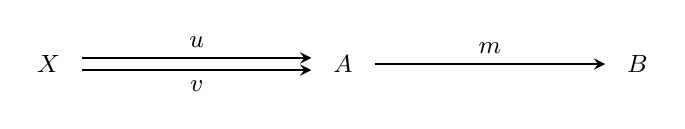
\begin{tikzpicture}[
		scale=1.1,
		every node/.style={font=\small},
		>=stealth
		]
		
		\node (X) at (0,0) {$X$};
		\node (A) at (3.4,0) {$A$};
		\node (B) at (6.8,0) {$B$};
		
		\draw[->,thick]
		([xshift=4pt,yshift=2pt]X.east) --
		node[above] {$u$}
		([xshift=-4pt,yshift=2pt]A.west);
		
		\draw[->,thick]
		([xshift=4pt,yshift=-2pt]X.east) --
		node[below] {$v$}
		([xshift=-4pt,yshift=-2pt]A.west);
		
		\draw[->,thick]
		([xshift=4pt]A.east) --
		node[above] {$m$}
		([xshift=-4pt]B.west);
		
	\end{tikzpicture}
\end{center}

La hipòtesi afirma que els dos camins de \(X\) a \(B\) coincideixen; la conclusió afirma que les dues aplicacions de \(X\) a \(A\) ja eren iguals. Equivalentment, pel contrarecíproc, tenim
\[
u\ne v\Longrightarrow m\circ u\ne m\circ v.
\]
Així, un monomorfisme no identifica dos elements generalitzats diferents de \(A\) que tinguin el mateix estadi \(X\).

\begin{definicio}[Epimorfisme]\index{Epimorfisme}\label{def:epimorfisme}
Una aplicació \(e\) és un \emph{epimorfisme} si es pot cancel·lar per la dreta. Formalment,
\[
\begin{aligned}
\operatorname{Epi}(e)
\iff {}&
\exists A\,\exists B\,\Bigl(
\Dom(e,A)\land\Cod(e,B)
\\
&{}\land
\forall Y\,\forall u\,\forall v\,
\Bigl(
\Dom(u,B)\land\Cod(u,Y)
\\
&\qquad{}\land\Dom(v,B)\land\Cod(v,Y)
\\
&\qquad{}\land\exists h\,
\bigl(\Com(e,u,h)\land\Com(e,v,h)\bigr)
\Rightarrow u=v
\Bigr)
\Bigr).
\end{aligned}
\]
\end{definicio}

\begin{notacio}[Fletxa epimòrfica]\label{not:epi}
Si \(e:A\to B\) i \(\operatorname{Epi}(e)\), escriurem
\[
e:A\twoheadrightarrow B.
\]
Amb aquesta notació, la condició d'epimorfisme s'abreuja així: per a totes les aplicacions paral·leles \(u,v:B\to Y\),
\[
u\circ e=v\circ e\Longrightarrow u=v.
\]
\end{notacio}

La situació dual de l'anterior és
\begin{center}
	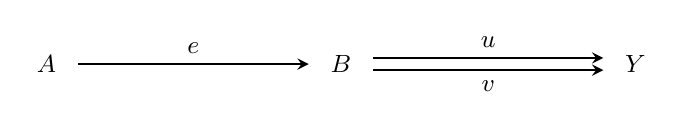
\begin{tikzpicture}[
		scale=1.1,
		every node/.style={font=\small},
		>=stealth
		]
		
		\node (A) at (0,0) {$A$};
		\node (B) at (3.4,0) {$B$};
		\node (Y) at (6.8,0) {$Y$};
		
		\draw[->,thick]
		([xshift=4pt]A.east) --
		node[above] {$e$}
		([xshift=-4pt]B.west);
		
		\draw[->,thick]
		([xshift=4pt,yshift=2pt]B.east) --
		node[above] {$u$}
		([xshift=-4pt,yshift=2pt]Y.west);
		
		\draw[->,thick]
		([xshift=4pt,yshift=-2pt]B.east) --
		node[below] {$v$}
		([xshift=-4pt,yshift=-2pt]Y.west);
		
	\end{tikzpicture}
\end{center}

En aquest cas es comparen dues aplicacions que tenen el mateix domini \(B\) i, dualment, també el mateix codomini \(Y\). Si els dos camins d'\(A\) a \(Y\) coincideixen després de precompondre \(u\) i \(v\) amb \(e\), aleshores \(u=v\). Així, un epimorfisme determina les aplicacions que surten de \(B\) cap a un codomini fix.

\begin{definicio}[Bimorfisme]\index{Bimorfisme}\label{def:bimorfisme}
Una aplicació és un \emph{bimorfisme} si és alhora un monomorfisme i un epimorfisme. Formalment,
\[
\operatorname{Bimor}(f)
\iff
\operatorname{Mono}(f)\land\operatorname{Epi}(f).
\]
\end{definicio}

A la \hyperref[prop:bimorfisme-isomorfisme]{proposició~\ref*{prop:bimorfisme-isomorfisme}} demostrarem que, amb els axiomes d'aquest capítol, els bimorfismes són precisament els isomorfismes. Fins que no s'hagi demostrat aquest resultat, no identificarem les dues nocions.

\begin{proposicio}\label{prop:identitat-mono-epi}
Per a qualsevol conjunt \(A\), l'aplicació identitat
\[
\id_A:A\to A
\]
és un monomorfisme i un epimorfisme.
\end{proposicio}

\begin{prova}
Si \(\id_A\circ u=\id_A\circ v\), les lleis de neutralitat donen \(u=v\); per tant, \(\id_A\) és un monomorfisme. De la mateixa manera, si \(u\circ\id_A=v\circ\id_A\), obtenim \(u=v\), i \(\id_A\) és un epimorfisme.
\end{prova}

\begin{proposicio}\label{prop:composicio-mono-epi}
La composició de monomorfismes és un monomorfisme, i la composició d'epimorfismes és un epimorfisme.
\end{proposicio}

\begin{prova}
Siguin
\[
A\xrightarrow{m}B\xrightarrow{n}C
\]
dos monomorfismes. Si
\[
(n\circ m)\circ u=(n\circ m)\circ v,
\]
per l'associativitat tenim
\[
n\circ(m\circ u)=n\circ(m\circ v).
\]
Com que \(n\) és un monomorfisme, \(m\circ u=m\circ v\); i com que \(m\) també és un monomorfisme, \(u=v\). Per tant, \(n\circ m\) és un monomorfisme.

El cas dels epimorfismes és dual. Si \(e:A\to B\) i \(d:B\to C\) són epimorfismes i
\[
u\circ(d\circ e)=v\circ(d\circ e),
\]
l'associativitat dona
\[
(u\circ d)\circ e=(v\circ d)\circ e.
\]
Com que \(e\) és un epimorfisme, \(u\circ d=v\circ d\), i com que \(d\) és un epimorfisme, \(u=v\).
\end{prova}

\begin{proposicio}\label{prop:isomorfisme-mono-epi}
Tot isomorfisme és un monomorfisme i un epimorfisme.
\end{proposicio}

\begin{prova}
Sigui \(f:A\to B\) un isomorfisme i sigui \(f^{-1}:B\to A\) la seva inversa. Si \(f\circ u=f\circ v\), component per l'esquerra amb \(f^{-1}\) obtenim
\[
u=(f^{-1}\circ f)\circ u=(f^{-1}\circ f)\circ v=v.
\]
Per tant, \(f\) és un monomorfisme.

Si \(u\circ f=v\circ f\), component per la dreta amb \(f^{-1}\) obtenim
\[
u=u\circ(f\circ f^{-1})=v\circ(f\circ f^{-1})=v.
\]
Per tant, \(f\) és un epimorfisme.
\end{prova}

\begin{definicio}[Secció i retracció]\index{Secció i retracció}\label{def:seccio-retraccio}
Siguin \(s:A\to B\) i \(r:B\to A\). Direm que \(s\) és una \emph{secció} de \(r\), i que \(r\) és una \emph{retracció} de \(s\), si
\[
r\circ s=\id_A.
\]
Formalment, definim primer la relació entre les dues aplicacions:
\[
\begin{aligned}
\operatorname{SeccioDe}(s,r)
\iff
\exists A\,\exists B\,\Bigl(&
\Dom(s,A)\land\Cod(s,B)
\\
&{}\land\Dom(r,B)\land\Cod(r,A)
\land\Com(s,r,A)
\Bigr).
\end{aligned}
\]
A partir d'aquesta relació, les dues propietats unàries s'abreugen per
\[
\operatorname{Seccio}(s)
\iff
\exists r\,\operatorname{SeccioDe}(s,r),
\qquad
\operatorname{Retraccio}(r)
\iff
\exists s\,\operatorname{SeccioDe}(s,r).
\]
\end{definicio}

\begin{notacio}[Triangle de secció i retracció]\label{not:seccio-retraccio}
La condició \(r\circ s=\id_A\) es representa mitjançant el triangle commutatiu
\begin{center}
\begin{tikzpicture}[scale=1.1, every node/.style={font=\small}]
  \node (A1) at (0,1.7) {\(A\)};
  \node (B) at (3.3,1.7) {\(B\)};
  \node (A2) at (3.3,0) {\(A\)};
  \draw[-{Stealth[scale=1.15]}, thick] (A1) -- node[above] {\(s\)} (B);
  \draw[-{Stealth[scale=1.15]}, thick] (B) -- node[right] {\(r\)} (A2);
  \draw[-{Stealth[scale=1.15]}, thick] (A1) -- node[below left] {\(\id_A\)} (A2);
\end{tikzpicture}
\end{center}
\end{notacio}

\begin{proposicio}\label{prop:seccio-mono-retraccio-epi}
Tota secció és un monomorfisme i tota retracció és un epimorfisme.
\end{proposicio}

\begin{prova}
Suposem que \(r\circ s=\id_A\). Si \(s\circ u=s\circ v\), component per l'esquerra amb \(r\) obtenim
\[
u=(r\circ s)\circ u=(r\circ s)\circ v=v.
\]
Així, \(s\) és un monomorfisme.

Si \(u\circ r=v\circ r\), component per la dreta amb \(s\) obtenim
\[
u=u\circ(r\circ s)=v\circ(r\circ s)=v.
\]
Per tant, \(r\) és un epimorfisme.
\end{prova}

\begin{observacio}[Monomorfismes i epimorfismes escindits]\index{Monomorfisme escindit}\index{Epimorfisme escindit}\label{obs:escindits}
Siguin \(f:A\to B\) i \(g:B\to A\) tals que
\[
g\circ f=\id_A.
\]
Aleshores \(f\) és una secció de \(g\), i \(g\) és una retracció de \(f\). També direm que \(f\) és un \emph{monomorfisme escindit} i que \(g\) és un \emph{epimorfisme escindit}. Aquesta situació és intermèdia entre una aplicació qualsevol i un isomorfisme, perquè només s'exigeix una de les dues identitats d'inversió.

En la lectura clàssica, \(f\) insereix \(A\) en \(B\), i \(g\) permet recuperar cada element de \(A\) després d'aquesta inserció.

\begin{figure}[H]
  \centering
  \begin{tikzpicture}[scale=1.2, every node/.style={font=\small}]
    \node (A) at (0,0) {\(A\)};
    \node (B) at (3,0) {\(B\)};
    \draw[-{Stealth[scale=1.2]}, thick] (A) edge[bend left=20] node[above] {\(f\)} (B);
    \draw[-{Stealth[scale=1.2]}, thick] (B) edge[bend left=20] node[below] {\(g\)} (A);
    \draw[-{Stealth[scale=1.2]}, thick] (A) to [out=135,in=225,looseness=6] node[left] {\(\id_A\)} (A);
  \end{tikzpicture}
  \caption{Diagrama d'una secció i d'una retracció: la composició $g\circ f$ és la identitat d'$A$, però no s'exigeix que $f\circ g=\id_B$.}
  \label{fig:seccio-retraccio}
\end{figure}

\end{observacio}

Els epimorfismes escindits admeten una caracterització en termes d'elements generalitzats, que reforça la noció d'exhaustivitat i que serà el punt de partida de l'estudi de l'elecció.

\begin{definicio}[Aplicació exhaustiva sobre elements generalitzats]\index{Aplicació exhaustiva sobre elements generalitzats}\label{def:exhaustiva-generalitzada}
Una aplicació \(f\) és \emph{exhaustiva sobre elements generalitzats} si tot element generalitzat del seu codomini es factoritza a través de \(f\). Formalment,
\[
\begin{aligned}
\operatorname{ExhGen}(f)
\iff {}&
\exists A\,\exists B\,\Bigl(
\Dom(f,A)\land\Cod(f,B)
\\
&{}\land
\forall X\,\forall y\,\Bigl(
\Dom(y,X)\land\Cod(y,B)
\\
&\qquad{}\Rightarrow
\exists x\,\bigl(\Dom(x,X)\land\Cod(x,A)\land\Com(x,f,y)\bigr)
\Bigr)
\Bigr).
\end{aligned}
\]
\end{definicio}

\begin{notacio}[Exhaustivitat generalitzada]\label{not:exhaustiva-generalitzada}
En notació de fletxes, \(f:A\to B\) és exhaustiva sobre elements generalitzats si, per a tot estadi \(X\) i tot element generalitzat \(y:X\to B\), existeix un element generalitzat \(x:X\to A\) tal que
\[
f\circ x=y.
\]
És a dir, tot element generalitzat de \(B\) és una avaluació de \(f\): és de la forma \(f\circ x\) per a un element generalitzat \(x\) de \(A\) en el mateix estadi.
\end{notacio}

\begin{proposicio}[Exhaustivitat generalitzada i epimorfismes escindits]\label{prop:exhaustiva-generalitzada-escindit}
Sigui \(f:A\to B\). Són equivalents:
\begin{enumerate}
\item \(f\) és exhaustiva sobre elements generalitzats;
\item \(f\) té una secció, és a dir, existeix \(s:B\to A\) amb \(f\circ s=\id_B\);
\item \(f\) és un epimorfisme escindit.
\end{enumerate}
\end{proposicio}

\begin{prova}
L'equivalència entre (2) i (3) és la definició d'epimorfisme escindit.

\emph{(1) \(\Rightarrow\) (2).} Apliquem l'exhaustivitat generalitzada a l'estadi \(X=B\) i a l'element generalitzat \(\id_B:B\to B\). Obtenim una aplicació \(s:B\to A\) amb \(f\circ s=\id_B\), que és una secció de \(f\).

\emph{(2) \(\Rightarrow\) (1).} Sigui \(s\) una secció de \(f\), i sigui \(y:X\to B\) un element generalitzat qualsevol. Aleshores \(x:=s\circ y:X\to A\) compleix
\[
f\circ x=f\circ(s\circ y)=(f\circ s)\circ y=\id_B\circ y=y,
\]
de manera que \(y\) és l'avaluació \(f\circ x\). Per tant, \(f\) és exhaustiva sobre elements generalitzats.
\end{prova}

\begin{observacio}[Exhaustivitat generalitzada i exhaustivitat global]\label{obs:exhaustiva-generalitzada-global}
L'exhaustivitat sobre elements generalitzats és una condició més forta que l'exhaustivitat sobre els elements globals: la primera exigeix que tot element generalitzat \(y:X\to B\) sigui una avaluació de \(f\), per a qualsevol estadi \(X\), mentre que la segona només ho demana per als elements globals, és a dir, per a l'estadi terminal \(\mathbf1\). Per la proposició anterior, l'exhaustivitat generalitzada equival a l'existència d'una secció; és, doncs, una propietat almenys tan forta com ser epimorfisme, i possiblement més forta. La qüestió de si tot epimorfisme és exhaustiu sobre elements generalitzats ---és a dir, si tot epimorfisme és escindit--- no es decideix amb els axiomes actuals, i es reprendrà en estudiar l'axioma d'elecció.
\end{observacio}

\section{Parts d'un conjunt}\label{sec:parts}

Els monomorfismes permeten expressar la noció de part exclusivament mitjançant aplicacions.

\begin{definicio}[Part]\index{Part}\label{def:part}
Una \emph{part} d'un conjunt \(A\) és un monomorfisme amb codomini \(A\). Formalment,
\[
\operatorname{Part}(m,A)
\iff
\operatorname{Conj}(A)\land\operatorname{Mono}(m)\land\Cod(m,A).
\]
\end{definicio}

\begin{notacio}[Representació d'una part]\label{not:part}
Si \(\operatorname{Part}(m,A)\) i \(S=\dom(m)\), escriurem
\[
m:S\hookrightarrow A.
\]
Reservarem, per tant, la fletxa amb ganxo per indicar que un monomorfisme és considerat com una part del seu codomini. El conjunt \(S\) és el domini de la part i \(m\) especifica la manera com aquesta part està situada en \(A\).
\end{notacio}

Una part no és, per tant, només el seu domini. Dos monomorfismes amb el mateix domini i el mateix codomini poden situar el domini de maneres diferents dins del codomini.

\subsection{Inclusió de parts}\label{sec:inclusio-parts}

\begin{definicio}[Inclusió]\index{Inclusió}\label{def:inclusio}
Siguin \(m\) i \(n\) dues parts del mateix conjunt \(A\). Direm que \(m\) està \emph{inclosa} en \(n\) si es factoritza a través de \(n\). Formalment,
\[
\operatorname{Incl}(m,n,A)
\iff
\operatorname{Part}(m,A)\land\operatorname{Part}(n,A)
\land\exists k\,\Com(k,n,m).
\]
\end{definicio}

\begin{notacio}[Inclusió de parts]\label{not:inclusio}
Escriurem
\[
m\subseteq_A n
\]
com a abreviació de \(\operatorname{Incl}(m,n,A)\). Si \(m:S\hookrightarrow A\) i \(n:T\hookrightarrow A\), aquesta condició significa que existeix una aplicació \(k:S\to T\) tal que
\[
m=n\circ k.
\]
Geomètricament, la inclusió queda representada pel triangle commutatiu
\begin{center}
	\begin{tikzpicture}[scale=1.1, every node/.style={font=\small}, >=Stealth]
		\node (S) at (0,1.7) {$S$};
		\node (T) at (3.3,1.7) {$T$};
		\node (A) at (3.3,0) {$A$};
		
		\draw[->, thick, dashed]
		(S) -- node[above] {$k$} (T);
		
		\draw[{Hooks[right]}-{Stealth[scale=1.2]}, thick]
		(T) -- node[right] {$n$} (A);
		
		\draw[{Hooks[right]}-{Stealth[scale=1.2]}, thick]
		(S) -- node[below left] {$m$} (A);
	\end{tikzpicture}
\end{center}
La fletxa discontínua posa de relleu que \(k\) és determinada per la factorització.
\end{notacio}

\begin{proposicio}\label{prop:testimoni-inclusio}
Si \(m\subseteq_A n\), l'aplicació \(k\) que satisfà \(m=n\circ k\) és única. A més, \(k\) és un monomorfisme.
\end{proposicio}

\begin{prova}
Si \(m=n\circ k=n\circ k'\), com que \(n\) és un monomorfisme, tenim \(k=k'\).

Per demostrar que \(k\) és un monomorfisme, suposem que \(k\circ u=k\circ v\). Aleshores
\[
m\circ u=n\circ k\circ u=n\circ k\circ v=m\circ v.
\]
Com que \(m\) és un monomorfisme, \(u=v\).
\end{prova}

\section{Pertinença generalitzada}\label{sec:pertinenca-generalitzada}

La inclusió expressa la comparació entre dues parts. La pertinença generalitzada expressarà, també mitjançant una factorització, quan una aplicació amb codomini \(A\) passa a través d'una part de \(A\).

\begin{definicio}[Pertinença]\index{Pertinença}\label{def:pertinenca}
Un element generalitzat \(x\) pertany a una part \(m\) si es factoritza a través d'aquesta part. Formalment,
\[
\begin{aligned}
\operatorname{Pert}(x,X,m)
\iff {}&
\exists A\,\exists S\,\Bigl(
\operatorname{Part}(m,A)
\land\Dom(m,S)
\\
&{}\land\Dom(x,X)\land\Cod(x,A)
\\
&{}\land\exists \bar{x}\,\bigl(
\Dom(\bar{x},X)\land\Cod(\bar{x},S)
\land\Com(\bar{x},m,x)
\bigr)
\Bigr).
\end{aligned}
\]
\end{definicio}

\begin{notacio}[Pertinença a una part]\label{not:pertinenca-part}
Si \(m:S\hookrightarrow A\) i \(x:X\to A\), escriurem
\[
x\in_Xm
\]
com a abreviació de \(\operatorname{Pert}(x,X,m)\). Aquesta condició significa que existeix una aplicació \(\bar{x}:X\to S\) tal que
\[
x=m\circ\bar{x}.
\]
La factorització es representa mitjançant el triangle commutatiu
\begin{center}
\begin{tikzpicture}[scale=1.1, every node/.style={font=\small}, >=Stealth]
  \node (X) at (0,1.7) {$X$};
  \node (S) at (3.3,1.7) {$S$};
  \node (A) at (3.3,0) {$A$};

  \draw[->, thick, dashed]
    (X) -- node[above] {$\bar{x}$} (S);

  \draw[{Hooks[right]}-{Stealth[scale=1.2]}, thick]
    (S) -- node[right] {$m$} (A);

  \draw[->, thick]
    (X) -- node[below left] {$x$} (A);
\end{tikzpicture}
\end{center}
Quan l'estadi quedi determinat pel context, podrem escriure simplement \(x\in m\).
\end{notacio}

La pertinença no és una relació primitiva entre individus, sinó una propietat definida a partir de la composició d'aplicacions.

\begin{proposicio}\label{prop:testimoni-pertinenca}
Si \(x\in_Xm\), l'aplicació \(\bar{x}:X\to S\) que satisfà \(x=m\circ\bar{x}\) és única.
\end{proposicio}

\begin{prova}
Si
\[
x=m\circ\bar{x}=m\circ\bar{x}',
\]
com que \(m\) és un monomorfisme, \(\bar{x}=\bar{x}'\).
\end{prova}

\begin{proposicio}\label{prop:inclusio-pertinenca}
Siguin \(m:S\hookrightarrow A\) i \(n:T\hookrightarrow A\) dues parts de \(A\). Aleshores
\[
m\subseteq_A n
\]
si i només si, per a tot conjunt \(X\) i tota aplicació \(x:X\to A\),
\[
x\in_Xm\quad\Longrightarrow\quad x\in_Xn.
\]
\end{proposicio}

\begin{prova}
Suposem primer que \(m\subseteq_A n\). Existeix una aplicació \(k:S\to T\) tal que \(m=n\circ k\). Si \(x\in_Xm\), existeix una aplicació \(\bar{x}:X\to S\) tal que \(x=m\circ\bar{x}\). Les dues hipòtesis queden expressades pels triangles commutatius següents:

\begin{figure}[H]
	\centering
	\begin{tikzpicture}[scale=1.2, every node/.style={font=\small}]
		\node (U) at (0,1.5) {\(X\)};
		\node (S) at (2,1.5) {\(S\)};
		\node (T) at (4,1.5) {\(T\)};
		\node (A) at (2,0) {\(A\)};
		
		\draw[-{Stealth[scale=1.2]}, thick, dashed] (U) -- node[above] {\(\bar{x}\)} (S);
		\draw[-{Stealth[scale=1.2]}, thick, dashed] (S) -- node[above] {\(k\)} (T);
		\draw[-{Stealth[scale=1.2]}, thick] (U) -- node[below left] {\(x\)} (A);
		\draw[{Hooks[right]}-{Stealth[scale=1.2]}, thick] (S) -- node[left] {\(m\)} (A);
		\draw[{Hooks[right]}-{Stealth[scale=1.2]}, thick] (T) -- node[below right] {\(n\)} (A);
	\end{tikzpicture}
	\caption{Si \(x \in_X m\) i \(m \subseteq_A n\), el testimoni de \(x \in_X n\) és \(k \circ \bar{x}\).}
	\label{fig:fonamental}
\end{figure}

En compondre les dues fletxes discontínues obtenim
\[
x=m\circ\bar{x}
  =(n\circ k)\circ\bar{x}
  =n\circ(k\circ\bar{x}).
\]
Per tant, el triangle
\begin{center}
\begin{tikzpicture}[scale=1.1, every node/.style={font=\small}, >=Stealth]

    \node (A3) at (0,1.6) {$X$};
    \node (B3) at (3.2,1.6) {$T$};
    \node (C3) at (1.6,0) {$A$};

    \draw[->, thick, dashed]
        (A3) -- node[above] {$k\circ\bar{x}$} (B3);

    \draw[->, thick]
        (A3) -- node[left] {$x$} (C3);

    \draw[{Hooks[right]}-{Stealth[scale=1.2]}, thick]
        (B3) -- node[right] {$n$} (C3);

\end{tikzpicture}
\end{center}
commuta, i això significa que \(x\in_Xn\).

Recíprocament, suposem que, per a tot \(X\) i tot \(x:X\to A\), de \(x\in_Xm\) se segueix \(x\in_Xn\). Prenem
\[
X=S,
\qquad
x=m:S\hookrightarrow A.
\]
El triangle de l'esquerra mostra que \(m\in_Sm\), amb testimoni \(\id_S\). La hipòtesi proporciona llavors una aplicació \(k:S\to T\) que fa commutar el triangle de la dreta:

\begin{figure}[H]
	\centering
	\begin{tikzpicture}[scale=1.2, every node/.style={font=\small}]
		\node (U) at (0,1.5) {\(S\)};
		\node (S) at (2,1.5) {\(S\)};
		\node (T) at (4,1.5) {\(T\)};
		\node (A) at (2,0) {\(A\)};
		
		\draw[-{Stealth[scale=1.2]}, thick] (U) -- node[above] {\(\id_S\)} (S);
		\draw[-{Stealth[scale=1.2]}, thick, dashed] (S) -- node[above] {\(k\)} (T);
		\draw[{Hooks[right]}-{Stealth[scale=1.2]}, thick] (U) -- node[below left] {\(m\)} (A);
		\draw[{Hooks[right]}-{Stealth[scale=1.2]}, thick] (S) -- node[left] {\(m\)} (A);
		\draw[{Hooks[right]}-{Stealth[scale=1.2]}, thick] (T) -- node[below right] {\(n\)} (A);
	\end{tikzpicture}
\end{figure}

Aquest triangle expressa
\[
m=n\circ k,
\]
i, per definició, \(m\subseteq_A n\).
\end{prova}

La \hyperref[prop:inclusio-pertinenca]{proposició~\ref*{prop:inclusio-pertinenca}} és la forma estructural del criteri d'inclusió: una part està inclosa en una altra exactament quan tots els seus elements generalitzats pertanyen també a l'altra.

\section{Parts equivalents i subconjunts}\label{sec:parts-equivalents}

Abans de comparar dues parts, observem que el domini d'una part es pot substituir per un conjunt isomorf sense perdre la propietat de ser una part.

\begin{proposicio}[Reparametrització isomorfa d'una part]\label{prop:reparametritzacio-part}
Siguin
\[
m:S\hookrightarrow A
\qquad\text{i}\qquad
t:T\xrightarrow{\sim}S.
\]
Aleshores
\[
m\circ t:T\hookrightarrow A
\]
és una part de \(A\).
\end{proposicio}

\begin{prova}
Tot isomorfisme és un monomorfisme per la \hyperref[prop:isomorfisme-mono-epi]{proposició~\ref*{prop:isomorfisme-mono-epi}}, i la composició de monomorfismes és un monomorfisme per la \hyperref[prop:composicio-mono-epi]{proposició~\ref*{prop:composicio-mono-epi}}. Per tant, \(m\circ t\) és un monomorfisme amb codomini \(A\), és a dir, una part de \(A\).

Geomètricament, la nova part és el camí exterior del triangle commutatiu
\begin{center}
\begin{tikzpicture}[scale=1.1, every node/.style={font=\small}, >=stealth]
  \node (T) at (0,1.7) {\(T\)};
  \node (S) at (3.3,1.7) {\(S\)};
  \node (A) at (3.3,0) {\(A\)};
  \draw[->, thick] (T) -- node[above] {\(\sim\)} node[below] {\(t\)} (S);
  \draw[{Hooks[right]}-{Stealth[scale=1.2]}, thick] (S) -- node[right] {\(m\)} (A);
  \draw[{Hooks[right]}-{Stealth[scale=1.2]}, thick] (T) -- node[below left] {\(m\circ t\)} (A);
\end{tikzpicture}
\end{center}
\end{prova}

\begin{definicio}[Equivalència de parts]\index{Equivalència de parts}\label{def:parts-equivalents}
Dues parts \(m\) i \(n\) de \(A\) són \emph{equivalents} si cadascuna es factoritza a través de l'altra. Formalment,
\[
\operatorname{EqPart}(m,n,A)
\iff
\operatorname{Incl}(m,n,A)\land\operatorname{Incl}(n,m,A).
\]
\end{definicio}

\begin{notacio}[Equivalència de parts]\label{not:equivalencia-parts}
Escriurem
\[
m\equiv_A n
\]
com a abreviació de \(\operatorname{EqPart}(m,n,A)\).
\end{notacio}

Siguin \(m:S\hookrightarrow A\) i \(n:T\hookrightarrow A\). Si \(m\equiv_A n\), existeixen aplicacions \(k:S\to T\) i \(t:T\to S\) tals que
\[
m=n\circ k,
\qquad
n=m\circ t.
\]
Les dues factoritzacions es representen simultàniament mitjançant el diagrama
\begin{center}
\begin{tikzpicture}[scale=1.1, every node/.style={font=\small}, >=Stealth]

  \node (S) at (0,1.8) {$S$};
  \node (T) at (4.0,1.8) {$T$};
  \node (A) at (2.0,0) {$A$};

  \draw[->, thick, dashed]
    ([yshift=2pt]S.east) --
    node[above] {$k$}
    ([yshift=2pt]T.west);

  \draw[->, thick, dashed]
    ([yshift=-2pt]T.west) --
    node[below] {$t$}
    ([yshift=-2pt]S.east);

  \draw[{Hooks[right]}-{Stealth[scale=1.2]}, thick]
    (S) -- node[below left] {$m$} (A);

  \draw[{Hooks[right]}-{Stealth[scale=1.2]}, thick]
    (T) -- node[below right] {$n$} (A);

\end{tikzpicture}
\end{center}

\begin{proposicio}\label{prop:parts-equivalents-isomorfisme}
Si \(m\equiv_A n\), les aplicacions \(k:S\to T\) i \(t:T\to S\) que testimonien les dues factoritzacions són isomorfismes inversos l'una de l'altra. En particular, existeix un únic isomorfisme \(k:S\to T\) tal que
\[
m=n\circ k.
\]
Recíprocament, l'existència d'un isomorfisme \(k:S\to T\) que satisfà aquesta igualtat implica \(m\equiv_A n\).
\end{proposicio}

\begin{prova}
Suposem que
\[
m=n\circ k,
\qquad
n=m\circ t.
\]
Aleshores
\[
n\circ(k\circ t)
=(n\circ k)\circ t
=m\circ t
=n
=n\circ\id_T.
\]
Com que \(n\) és un monomorfisme,
\[
k\circ t=\id_T.
\]
Anàlogament,
\[
m\circ(t\circ k)
=(m\circ t)\circ k
=n\circ k
=m
=m\circ\id_S,
\]
i, com que \(m\) és un monomorfisme,
\[
t\circ k=\id_S.
\]
Per tant, \(k\) i \(t\) són isomorfismes inversos. La unicitat de \(k\) és una conseqüència de la \hyperref[prop:testimoni-inclusio]{proposició~\ref*{prop:testimoni-inclusio}}.

Recíprocament, si \(k:S\to T\) és un isomorfisme i \(m=n\circ k\), tenim \(m\subseteq_A n\). Com que
\[
n=m\circ k^{-1},
\]
també \(n\subseteq_A m\), i per tant \(m\equiv_A n\).
\end{prova}

\begin{proposicio}\label{prop:equivalencia-parts}
Per a parts \(m,n,p\) d'un mateix conjunt \(A\), es compleixen les propietats següents:
\[
m\equiv_A m;
\]
\[
m\equiv_A n\Longrightarrow n\equiv_A m;
\]
\[
m\equiv_A n\land n\equiv_A p
\Longrightarrow
m\equiv_A p.
\]
\end{proposicio}

\begin{prova}
La primera propietat es testimonia amb l'aplicació identitat del domini de \(m\). La segona se segueix directament de la simetria de les dues factoritzacions que formen la definició de \(m\equiv_A n\).

Per a la tercera, la \hyperref[prop:parts-equivalents-isomorfisme]{proposició~\ref*{prop:parts-equivalents-isomorfisme}} proporciona isomorfismes
\[
k:\dom(m)\xrightarrow{\sim}\dom(n),
\qquad
\ell:\dom(n)\xrightarrow{\sim}\dom(p)
\]
compatibles amb les tres parts. La composició \(\ell\circ k\) és un isomorfisme i proporciona la factorització de \(m\) a través de \(p\). La seva inversa proporciona la factorització de \(p\) a través de \(m\). Per tant, \(m\equiv_A p\).
\end{prova}

\begin{observacio}[Recuperació metalingüística dels subconjunts]\label{obs:subconjunt-metallenguatge}
Fixem un conjunt \(A\). Una mateixa part estructural pot ser representada per monomorfismes
\[
m:S\hookrightarrow A
\]
amb dominis diferents però isomorfs. La notació \(m\equiv_A n\) expressa que dues d'aquestes representacions determinen la mateixa manera de situar una part dins de \(A\), llevat d'un canvi isomorf del domini.

En el metallenguatge, podem recuperar la noció clàssica de \emph{subconjunt de \(A\)} considerant la classe de totes les parts de \(A\) equivalents a un representant donat. Aquesta classe no és, de moment, un conjunt intern de la teoria. En els raonaments treballarem amb una part concreta com a representant, i les proposicions anteriors garantiran que les propietats estructurals no depenen del representant escollit.
\end{observacio}

\section{Sumes de conjunts}\label{sec:suma}

\begin{definicio}[Suma]\index{Suma}\label{def:suma-conjunts}
Un conjunt \(S\), juntament amb aplicacions
\[
i_0:A_0\to S,
\qquad
i_1:A_1\to S,
\]
és una \emph{suma} dels conjunts \(A_0\) i \(A_1\) si compleix la propietat universal següent. Formalment,
\[
\begin{aligned}
&\operatorname{Suma}(S,i_0,i_1,A_0,A_1)
\\
\iff {}&
\operatorname{Conj}(S)
\land\Dom(i_0,A_0)\land\Cod(i_0,S)
\land\Dom(i_1,A_1)\land\Cod(i_1,S)
\\
&{}\land
\forall B\,\forall f_0\,\forall f_1\,
\Bigl(
\operatorname{Conj}(B)
\land\Dom(f_0,A_0)\land\Cod(f_0,B)
\\
&\qquad{}\land\Dom(f_1,A_1)\land\Cod(f_1,B)
\\
&\qquad{}\Rightarrow
\exists!h\,
\bigl(
\Dom(h,S)\land\Cod(h,B)
\land\Com(i_0,h,f_0)\land\Com(i_1,h,f_1)
\bigr)
\Bigr).
\end{aligned}
\]
\end{definicio}

\begin{notacio}[Suma i aplicació definida per casos]\label{not:suma}
Quan \(\operatorname{Suma}(S,i_0,i_1,A_0,A_1)\), representarem les dues \emph{injeccions} de la suma per dues fletxes que conflueixen en \(S\):
\[
A_0\xrightarrow{i_0}S\xleftarrow{i_1}A_1.
\]
Les aplicacions \(i_0\) i \(i_1\) s'anomenen \emph{injeccions} de la suma (o \emph{injeccions canòniques}). Reservem aquest terme per a les fletxes estructurals \(i_0,i_1\) d'una suma, i el terme \emph{inclusió} per als subobjectes \(S\hookrightarrow A\) i l'ordre entre parts (definició~\ref{def:inclusio}); són nocions distintes. En aquest punt les injeccions són simplement les fletxes de la propietat universal: encara \emph{no} sabem que siguin monomorfismes, cosa que dependrà de la disjunció de les sumes (definició~\ref{def:suma-disjunta} i axioma~\ref{ax:sumes-disjuntes}, capítol~\ref{cap:valors}). Per a \(f_0:A_0\to B\) i \(f_1:A_1\to B\), denotarem l'única aplicació proporcionada per la propietat universal per
\[
[f_0,f_1]:S\to B.
\]
Així, les fórmules \(\Com(i_0,[f_0,f_1],f_0)\) i \(\Com(i_1,[f_0,f_1],f_1)\) s'escriuen
\[
[f_0,f_1]\circ i_0=f_0,
\qquad
[f_0,f_1]\circ i_1=f_1.
\]
La propietat universal queda representada pel diagrama commutatiu
\begin{center}
\begin{tikzpicture}[scale=1.05, every node/.style={font=\small}, >=Stealth]
  \node (A0) at (0,2.1) {\(A_0\)};
  \node (S)  at (3.4,2.1) {\(S\)};
  \node (A1) at (6.8,2.1) {\(A_1\)};
  \node (B)  at (3.4,0) {\(B\)};

  \draw[->, thick] (A0) -- node[above] {\(i_0\)} (S);
  \draw[->, thick] (A1) -- node[above] {\(i_1\)} (S);
  \draw[->, thick] (A0) -- node[below left] {\(f_0\)} (B);
  \draw[->, thick] (A1) -- node[below right] {\(f_1\)} (B);
  \draw[->, thick, dashed] (S) -- node[right] {\([f_0,f_1]\)} (B);
\end{tikzpicture}
\end{center}
La fletxa discontínua posa de relleu que l'aplicació \([f_0,f_1]\) existeix i és única.
\end{notacio}

\begin{proposicio}[Extensionalitat de la definició per casos]\label{prop:extensionalitat-suma}
Si
\[
A_0\xrightarrow{i_0}S\xleftarrow{i_1}A_1
\]
és una suma i \(h:S\to B\), aleshores
\[
h=[h\circ i_0,h\circ i_1].
\]
En particular, per a dues aplicacions \(h,k:S\to B\),
\[
h=k
\quad\Longleftrightarrow\quad
h\circ i_0=k\circ i_0
\ \land\ 
h\circ i_1=k\circ i_1.
\]
\end{proposicio}

\begin{prova}
Les aplicacions \(h\) i \([h\circ i_0,h\circ i_1]\) tenen les mateixes composicions amb \(i_0\) i \(i_1\). La unicitat de la propietat universal implica
\[
h=[h\circ i_0,h\circ i_1].
\]
La segona afirmació se segueix aplicant aquesta identitat a \(h\) i a \(k\).
\end{prova}



\begin{axioma}[Existència de sumes]\label{ax:sumes}
Tot parell de conjunts té una suma. Formalment,
\[
\begin{aligned}
\forall A_0\,\forall A_1\,\Bigl(&
\operatorname{Conj}(A_0)\land\operatorname{Conj}(A_1)
\\
&{}\Rightarrow
\exists S\,\exists i_0\,\exists i_1\,
\operatorname{Suma}(S,i_0,i_1,A_0,A_1)
\Bigr).
\end{aligned}
\]
\end{axioma}

\begin{notacio}[Suma escollida]\label{not:suma-escollida}
Fixarem una suma de \(A_0\) i \(A_1\), que denotarem per \(A_0+A_1\), i escriurem
\[
i_0:A_0\to A_0+A_1,
\qquad
i_1:A_1\to A_0+A_1
\]
per a les injeccions escollides.
\end{notacio}

\begin{observacio}[Lectura clàssica de la suma i definició per casos]\label{ex:suma-classica}
En la teoria clàssica de conjunts, una suma es pot construir mitjançant dues còpies disjuntes dels conjunts:
\[
A_0+A_1
=
\bigl(\{0\}\times A_0\bigr)
\cup
\bigl(\{1\}\times A_1\bigr).
\]
Aquesta expressió pertany al metallenguatge i no és la definició formal de la suma dins de la teoria. Les etiquetes \(0\) i \(1\) només serveixen per distingir les dues còpies.

Donades aplicacions \(f_0:A_0\to B\) i \(f_1:A_1\to B\), l'aplicació
\[
[f_0,f_1]:A_0+A_1\to B
\]
es defineix per casos:
\[
[f_0,f_1](0,a)=f_0(a),
\qquad
[f_0,f_1](1,b)=f_1(b).
\]
La propietat universal expressa estructuralment que aquesta és l'única aplicació que actua com \(f_0\) sobre la primera còpia i com \(f_1\) sobre la segona.
\end{observacio}

\begin{proposicio}[Unicitat de la suma]\label{prop:suma-unica}
Dues sumes dels mateixos conjunts són isomorfes mitjançant un únic isomorfisme que conserva les injeccions.
\end{proposicio}

\begin{prova}
Siguin
\[
A_0\xrightarrow{i_0}S\xleftarrow{i_1}A_1
\]
i
\[
A_0\xrightarrow{j_0}T\xleftarrow{j_1}A_1
\]
dues sumes. Per la propietat universal de \(S\), existeix una única aplicació \(u:S\to T\) tal que
\[
u\circ i_0=j_0,
\qquad
u\circ i_1=j_1.
\]
Anàlogament, existeix una única aplicació \(v:T\to S\) tal que
\[
v\circ j_0=i_0,
\qquad
v\circ j_1=i_1.
\]
Les aplicacions \(v\circ u\) i \(\id_S\) tenen les mateixes composicions amb \(i_0\) i \(i_1\). Per la unicitat de la propietat universal,
\[
v\circ u=\id_S.
\]
De la mateixa manera,
\[
u\circ v=\id_T.
\]
Per tant, \(u\) és un isomorfisme. La seva unicitat forma part de la mateixa propietat universal.
\end{prova}

\begin{definicio}[Cograf]\index{Cograf}\label{def:cograf}
El \emph{cograf} d'una aplicació \(f:A\to B\) és l'aplicació de la suma \(A+B\) en \(B\) determinada per \(f\) i la identitat de \(B\). Formalment,
\[
\begin{aligned}
\operatorname{Cograf}(k,f)
\iff {}&
\exists A\,\exists B\,\exists S\,\exists i_0\,\exists i_1\,\Bigl(
\\
&\quad\Dom(f,A)\land\Cod(f,B)
\\
&\quad{}\land\operatorname{Suma}(S,i_0,i_1,A,B)
\\
&\quad{}\land\Dom(k,S)\land\Cod(k,B)
\\
&\quad{}\land\Com(i_0,k,f)\land\Com(i_1,k,B)
\Bigr).
\end{aligned}
\]
\end{definicio}

\begin{notacio}[Cograf]\label{not:cograf}
Denotarem el cograf de \(f\) per
\[
\kappa_f=[f,\id_B]:A+B\to B.
\]
La construcció queda representada pel diagrama commutatiu
\begin{center}
\begin{tikzpicture}[scale=1.05, every node/.style={font=\small}, >=Stealth]
  \node (A)  at (0,2.1) {\(A\)};
  \node (AB) at (3.4,2.1) {\(A+B\)};
  \node (Bt) at (6.8,2.1) {\(B\)};
  \node (Bb) at (3.4,0) {\(B\)};

  \draw[->, thick] (A) -- node[above] {\(i_0\)} (AB);
  \draw[->, thick] (Bt) -- node[above] {\(i_1\)} (AB);
  \draw[->, thick] (A) -- node[below left] {\(f\)} (Bb);
  \draw[->, thick] (Bt) -- node[below right] {\(\id_B\)} (Bb);
  \draw[->, thick, dashed] (AB) -- node[right] {\(\kappa_f\)} (Bb);
\end{tikzpicture}
\end{center}
Així,
\[
\kappa_f\circ i_0=f,
\qquad
\kappa_f\circ i_1=\id_B.
\]
\end{notacio}

\begin{observacio}[Lectura clàssica del cograf]\label{obs:cograf-classic}
En la representació clàssica de \(A+B\) com dues còpies disjuntes, el cograf envia la còpia d'un element \(a\in A\) al seu valor \(f(a)\in B\) i deixa fixa la còpia de cada element \(b\in B\). D'aquesta manera, els conjunts \(A\) i \(B\) apareixen situats un al costat de l'altre, i la branca corresponent a \(A\) recupera el diagrama intern de l'aplicació \(f\): de cada element del domini surt una fletxa cap al seu valor.
\end{observacio}

\begin{proposicio}\label{prop:cograf-retraccio}
El cograf \(\kappa_f\) és una retracció de la segona injecció \(i_1:B\to A+B\). En particular, \(\kappa_f\) és un epimorfisme i \(i_1\) és un monomorfisme. Simètricament, si existeix alguna aplicació \(g\colon B\to A\), el cograf \([\id_A,g]\colon A+B\to A\) és una retracció de \(i_0\), que és aleshores un monomorfisme.
\end{proposicio}

\begin{prova}
Per la definició de \([f,\id_B]\),
\[
\kappa_f\circ i_1=\id_B.
\]
La conclusió se segueix de la \hyperref[prop:seccio-mono-retraccio-epi]{proposició~\ref*{prop:seccio-mono-retraccio-epi}}; el cas de \(i_0\) és idèntic amb \([\id_A,g]\circ i_0=\id_A\). Observeu que l'argument necessita una aplicació entre els dos sumands: que les injeccions siguin monomorfismes \emph{en general} dependrà de la disjunció de les sumes (capítol~\ref{cap:valors}).
\end{prova}

\subsection{El conjunt \texorpdfstring{\(\mathbf2\)}{2}}\label{dos-oficial}

\begin{notacio}[El conjunt \(\mathbf2\) i els valors distingits]\label{not:dos}
Denotarem per \(\mathbf2\) la suma escollida \(\mathbf1+\mathbf1\):
\[
\mathbf2=\mathbf1+\mathbf1.
\]
Denotarem les dues injeccions per
\[
0:\mathbf1\to\mathbf2,
\qquad
1:\mathbf1\to\mathbf2.
\]
L'aplicació \(1\) serà la part distingida que intervindrà en l'axioma de representació.
\end{notacio}

\begin{corollari}\label{prop:zero-u-mono}
Les aplicacions \(0\) i \(1\) són monomorfismes.
\end{corollari}

\begin{prova}
La propietat universal de la suma determina una aplicació
\[
[\id_{\mathbf1},\id_{\mathbf1}]:\mathbf2\to\mathbf1.
\]
Aquesta aplicació és una retracció tant de \(0\) com de \(1\), perquè
\[
[\id_{\mathbf1},\id_{\mathbf1}]\circ0=\id_{\mathbf1}
\]
i
\[
[\id_{\mathbf1},\id_{\mathbf1}]\circ1=\id_{\mathbf1}.
\]
Per la \hyperref[prop:seccio-mono-retraccio-epi]{proposició~\ref*{prop:seccio-mono-retraccio-epi}}, \(0\) i \(1\) són monomorfismes.
\end{prova}

\begin{observacio}[Una aplicació de la suma cap a \(\mathbf2\)]\label{ex:suma-cap-dos}
Per a qualssevol conjunts \(A\) i \(B\), la propietat universal de la suma determina l'aplicació
\[
[0\circ {!}_A,1\circ {!}_B]:A+B\to\mathbf2.
\]
Aquesta aplicació és constant amb valor \(0\) sobre el sumand \(A\) i constant amb valor \(1\) sobre el sumand \(B\):
\[
[0\circ {!}_A,1\circ {!}_B]\circ i_0=0\circ {!}_A,
\]
\[
[0\circ {!}_A,1\circ {!}_B]\circ i_1=1\circ {!}_B.
\]
En la lectura clàssica, indica de quin dels dos sumands prové cada element de \(A+B\).
\end{observacio}

\begin{observacio}[Aplicacions de \(\mathbf2\) en un conjunt]\label{obs:dos-cap-a}
Donar una aplicació \(h:\mathbf2\to A\) equival a donar dues aplicacions
\[
a_0:\mathbf1\to A,
\qquad
a_1:\mathbf1\to A.
\]
En efecte, la propietat universal de \(\mathbf2=\mathbf1+\mathbf1\) determina l'aplicació
\[
[a_0,a_1]:\mathbf2\to A
\]
caracteritzada per
\[
[a_0,a_1]\circ0=a_0,
\qquad
[a_0,a_1]\circ1=a_1.
\]
Així, en la lectura clàssica, una aplicació de \(\mathbf2\) en \(A\) selecciona un parell ordenat d'elements de \(A\), que no han de ser necessàriament diferents.
\end{observacio}


\section{Representació de les parts}\label{representacio}

La pertinença a una part es pot convertir en una aplicació cap a \(\mathbf2\). Aquesta possibilitat no es dedueix dels axiomes anteriors i s'introdueix com un axioma nou.

\begin{definicio}[Aplicació característica]\index{Aplicació característica}\index{Classificador de parts}\label{def:caracteristica}
Una aplicació \(\chi\) és \emph{característica} d'una part \(m\) de \(A\) si classifica exactament els elements generalitzats que es factoritzen a través de \(m\). Formalment,
\[
\begin{aligned}
\operatorname{Car}(\chi,m,A)
\iff {}&
\operatorname{Part}(m,A)\land\Dom(\chi,A)\land\Cod(\chi,\mathbf2)
\\
&{}\land
\forall X\,\forall x\,
\Bigl(
\operatorname{Conj}(X)\land\Dom(x,X)\land\Cod(x,A)
\\
&\qquad{}\Rightarrow
\bigl(
\operatorname{Pert}(x,X,m)
\Longleftrightarrow
\chi\circ x=1\circ {!}_X
\bigr)
\Bigr).
\end{aligned}
\]
\end{definicio}

\begin{axioma}[Representació de les parts]\label{ax:representacio}
Tota part té una única aplicació característica, i tota aplicació cap a \(\mathbf2\) és la característica d'alguna part. Formalment,
\[
\begin{aligned}
\forall A\,\forall m\,\Bigl(&
\operatorname{Part}(m,A)
\Rightarrow
\exists!\chi\,\operatorname{Car}(\chi,m,A)
\Bigr),
\end{aligned}
\]
i
\[
\begin{aligned}
\forall A\,\forall\varphi\,\Bigl(&
\operatorname{Conj}(A)\land\Dom(\varphi,A)\land\Cod(\varphi,\mathbf2)
\\
&{}\Rightarrow
\exists m\,\operatorname{Car}(\varphi,m,A)
\Bigr).
\end{aligned}
\]
\end{axioma}

\begin{observacio}[Tres unicitats que no s'han de confondre]\label{obs:tres-unicitats}
L'axioma parla de dues unicitats diferents, i convé separar-les d'una tercera que no afirma. (i)~\emph{Unicitat de la característica:} per a cada monomorfisme \(m\), l'aplicació \(\chi\) amb \(\operatorname{Car}(\chi,m,A)\) és única com a fletxa, perquè la condició \(x\in_Xm\iff\chi\circ x=1\circ{!}_X\) la determina sobre tots els elements generalitzats d'\(A\). (ii)~\emph{Existència, però no unicitat, de la part:} per a cada \(\varphi\colon A\to\mathbf2\) existeix algun \(m\) amb \(\operatorname{Car}(\varphi,m,A)\), però no és únic com a fletxa: si \(m\colon S\hookrightarrow A\) ho compleix i \(u\colon S'\to S\) és un isomorfisme, \(m\circ u\) també ho compleix, perquè té els mateixos elements generalitzats. El que és únic és la \emph{classe d'equivalència} de la part: dues parts amb la mateixa característica tenen els mateixos elements generalitzats i són equivalents (proposició~\ref{prop:inclusio-pertinenca} en els dos sentits), i aleshores els seus dominis són isomorfs per un únic isomorfisme compatible amb les dues fletxes (proposició~\ref{prop:parts-equivalents-isomorfisme}). (iii)~\emph{Igualtat de fletxes:} que \(m\equiv_An\) no vol dir \(m=n\). En resum: les aplicacions \(A\to\mathbf2\) estan en correspondència bijectiva amb les \emph{classes} de parts equivalents d'\(A\), no amb les parts com a fletxes; és la mateixa situació que amb els subconjunts clàssics, que corresponen a les classes i no a les inclusions concretes (observació~\ref{obs:subconjunt-metallenguatge}).
\end{observacio}

\begin{notacio}[Aplicació característica]\label{not:caracteristica}
Si \(\operatorname{Car}(\chi,m,A)\), denotarem l'única aplicació característica per
\[
\chi_m:A\to\mathbf2.
\]
La seva propietat característica s'escriu
\[
x\in_Xm
\quad\Longleftrightarrow\quad
\chi_m\circ x=1\circ {!}_X.
\]
\end{notacio}

La factorització que expressa la pertinença \(x\in_Xm\) es representa mitjançant el triangle commutatiu
\begin{center}
\begin{tikzpicture}[scale=1.1, every node/.style={font=\small}, >=Stealth]
  \node (X) at (0,1.8) {\(X\)};
  \node (S) at (3.5,1.8) {\(S\)};
  \node (A) at (3.5,0) {\(A\)};

  \draw[->, thick, dashed] (X) -- node[above] {\(\bar{x}\)} (S);
  \draw[->, thick] (X) -- node[below left] {\(x\)} (A);
  \draw[{Hooks[right]}-{Stealth[scale=1.2]}, thick] (S) -- node[right] {\(m\)} (A);
\end{tikzpicture}
\end{center}
on \(x=m\circ\bar{x}\). Com que \(m\) és un monomorfisme, el testimoni \(\bar{x}\), quan existeix, és únic.

Prenent \(x=m:S\to A\) i \(\bar{x}=\id_S\), obtenim
\[
\chi_m\circ m=1\circ {!}_S.
\]
Aquesta igualtat queda representada pel quadrat commutatiu
\begin{center}
\begin{tikzpicture}[scale=1.1, every node/.style={font=\small}, >=Stealth]
  \node (S) at (0,1.9) {\(S\)};
  \node (One) at (3.8,1.9) {\(\mathbf1\)};
  \node (A) at (0,0) {\(A\)};
  \node (Two) at (3.8,0) {\(\mathbf2\)};

  \draw[->, thick] (S) -- node[above] {\({!}_S\)} (One);
  \draw[{Hooks[right]}-{Stealth[scale=1.2]}, thick] (S) -- node[left] {\(m\)} (A);
  \draw[{Hooks[right]}-{Stealth[scale=1.2]}, thick] (One) -- node[right] {\(1\)} (Two);
  \draw[->, thick] (A) -- node[below] {\(\chi_m\)} (Two);
\end{tikzpicture}
\end{center}
La propietat característica afirma que una aplicació \(x:X\to A\) es factoritza a través de \(m\) si i només si la composició \(\chi_m\circ x\) coincideix amb \(1\circ {!}_X\). Al \hyperref[teo:quadrat-caracteristic]{teorema~\ref*{teo:quadrat-caracteristic}} veurem que aquesta propietat diu exactament que el quadrat anterior és un pullback.

\begin{observacio}[Distingir elements mitjançant una aplicació característica]\label{obs:caracteristica-distingeix}
Siguin \(x,y:X\to A\) dos elements generalitzats. Si
\[
x\in_Xm
\qquad\text{i}\qquad
y\notin_Xm,
\]
aleshores
\[
\chi_m\circ x\neq\chi_m\circ y.
\]
En efecte, la primera condició implica \(\chi_m\circ x=1\circ {!}_X\), mentre que la segona implica \(\chi_m\circ y\neq1\circ {!}_X\).

En particular, quan \(X=\mathbf1\), l'aplicació característica recupera la noció clàssica de distingir dos elements d'un conjunt segons si pertanyen o no a una part. Els axiomes establerts fins aquí només afirmen que un element que no pertany a la part no és enviat al valor distingit \(1\); encara no afirmen que hagi de ser enviat necessàriament a \(0\).
\end{observacio}

L'axioma es formula per a tots els elements generalitzats. No afirma només quins punts globals pertanyen a una part, sinó quines aplicacions \(X\to A\) es factoritzen a través d'ella, per a qualsevol estadi \(X\).

\begin{proposicio}\label{prop:caracteristica-determina-part}
Dues parts \(m\) i \(n\) de \(A\) són equivalents si i només si tenen la mateixa aplicació característica:
\[
m\equiv_A n
\quad\Longleftrightarrow\quad
\chi_m=\chi_n.
\]
\end{proposicio}

\begin{prova}
Suposem primer que \(\chi_m=\chi_n\). Per a qualsevol \(x:X\to A\),
\[
\begin{aligned}
x\in_X m
&\Longleftrightarrow \chi_m\circ x=1\circ {!}_X\\
&\Longleftrightarrow \chi_n\circ x=1\circ {!}_X\\
&\Longleftrightarrow x\in_X n.
\end{aligned}
\]
Per la \hyperref[prop:inclusio-pertinenca]{proposició~\ref*{prop:inclusio-pertinenca}}, tenim \(m\subseteq_A n\) i \(n\subseteq_A m\). Per tant, \(m\equiv_A n\).

Recíprocament, suposem que \(m\equiv_A n\). La mateixa proposició implica que, per a qualsevol \(x:X\to A\),
\[
x\in_Xm\quad\Longleftrightarrow\quad x\in_Xn.
\]
Per tant, \(\chi_n\) satisfà la condició característica de \(m\). La unicitat establerta per l'axioma de representació implica
\[
\chi_m=\chi_n.
\]
\end{prova}

\begin{proposicio}\label{prop:caracteristica-total}
La característica de la part total \(\id_A:A\hookrightarrow A\) és l'aplicació constant
\[
1\circ {!}_A:A\to\mathbf2.
\]
\end{proposicio}

\begin{prova}
Per a tota aplicació \(x:X\to A\), tenim \(x\in_X\id_A\), amb testimoni \(x\). A més,
\[
(1\circ {!}_A)\circ x
=1\circ({!}_A\circ x)
=1\circ {!}_X.
\]
La unicitat de l'aplicació característica dona el resultat.
\end{prova}

\begin{proposicio}\label{prop:bimorfisme-isomorfisme}
Tot bimorfisme és un isomorfisme.
\end{proposicio}

\begin{prova}
Sigui \(f:A\to B\) un monomorfisme i un epimorfisme. Com que és un monomorfisme, podem considerar-lo una part de \(B\). Sigui
\[
\chi_f:B\to\mathbf2
\]
la seva aplicació característica.

La mateixa aplicació \(f:A\to B\) pertany a la part \(f\), amb testimoni \(\id_A\). Per tant,
\[
\chi_f\circ f=1\circ {!}_A.
\]
D'altra banda,
\[
(1\circ {!}_B)\circ f=1\circ {!}_A.
\]
Com que \(f\) és un epimorfisme,
\[
\chi_f=1\circ {!}_B.
\]
Així,
\[
\chi_f\circ\id_B=1\circ {!}_B,
\]
i l'axioma de representació implica
\[
\id_B\in_B f.
\]
Per tant, existeix una aplicació \(g:B\to A\) tal que
\[
f\circ g=\id_B.
\]
Finalment,
\[
f\circ(g\circ f)=(f\circ g)\circ f=f=f\circ\id_A.
\]
Com que \(f\) és un monomorfisme,
\[
g\circ f=\id_A.
\]
Per tant, \(g\) és la inversa de \(f\), i \(f\) és un isomorfisme.
\end{prova}

\begin{corollari}\label{cor:isomorfisme-bimorfisme}
Una aplicació és un isomorfisme si i només si és un monomorfisme i un epimorfisme.
\end{corollari}

\begin{prova}
Una implicació és la \hyperref[prop:isomorfisme-mono-epi]{proposició~\ref*{prop:isomorfisme-mono-epi}} i l'altra és la \hyperref[prop:bimorfisme-isomorfisme]{proposició~\ref*{prop:bimorfisme-isomorfisme}}.
\end{prova}

\begin{observacio}[Injectivitat clàssica i monomorfismes]\label{obs:injectiva-mono}
En la teoria clàssica de conjunts, una aplicació \(f:A\to B\) és \emph{injectiva} si, per a tots els elements globals \(x,y:\mathbf1\to A\),
\[
f\circ x=f\circ y
\quad\Longrightarrow\quad
x=y.
\]
En aquesta observació, i en les següents, ometrem l'expressió \enquote{respecte dels elements globals} perquè queda incorporada a la definició clàssica.

Tot monomorfisme és injectiu. En efecte, només cal aplicar la definició de monomorfisme a les aplicacions \(x,y:\mathbf1\to A\).

Recíprocament, suposem que \(f\) és injectiva i que
\[
f\circ u=f\circ v
\]
per a dues aplicacions \(u,v:X\to A\). Per a tot element global \(x:\mathbf1\to X\), l'associativitat dona
\[
f\circ(u\circ x)=f\circ(v\circ x).
\]
La injectivitat de \(f\) implica
\[
u\circ x=v\circ x.
\]
Per l'\hyperref[ax:separacio-globals]{axioma de separació global}, \(u=v\). Per tant,
\[
\boxed{
 f\text{ és injectiva}
 \quad\Longleftrightarrow\quad
 f\text{ és un monomorfisme}.
}
\]
Aquesta equivalència explica per què els monomorfismes són la formulació estructural de la injectivitat.
\end{observacio}

\begin{observacio}[Exhaustivitat clàssica i epimorfismes]\label{obs:exhaustiva-epi}
En la teoria clàssica de conjunts, una aplicació \(f:A\to B\) és \emph{exhaustiva} si, per a tot element global \(y:\mathbf1\to B\), existeix un element global \(x:\mathbf1\to A\) tal que
\[
f\circ x=y.
\]

Sota l'\hyperref[ax:separacio-globals]{axioma de separació global}, tota aplicació exhaustiva és un epimorfisme. En efecte, suposem que \(u,v:B\to C\) compleixen
\[
u\circ f=v\circ f.
\]
Per a qualsevol element global \(y:\mathbf1\to B\), l'exhaustivitat proporciona \(x:\mathbf1\to A\) amb \(f\circ x=y\). Llavors
\[
\begin{aligned}
u\circ y
&=u\circ(f\circ x)\\
&=(u\circ f)\circ x\\
&=(v\circ f)\circ x\\
&=v\circ(f\circ x)\\
&=v\circ y.
\end{aligned}
\]
La separació global implica \(u=v\), i per tant \(f\) és un epimorfisme.

El recíproc ---que tot epimorfisme sigui exhaustiu sobre els elements globals--- no es pot demostrar amb els axiomes d'aquest capítol, perquè demana saber que un conjunt sense punts globals és inicial i que els dos valors \(0,1\colon\mathbf1\to\mathbf2\) són diferents, fets que no establirem fins al capítol~\ref{cap:valors}. Allà el demostrarem, amb la separació global i sense cap axioma d'elecció. Fins aleshores, i en tot el desenvolupament estructural, mantindrem separades les nocions d'epimorfisme i d'exhaustivitat sobre punts; la noció més forta, l'exhaustivitat sobre elements \emph{generalitzats}, sí que és estrictament més forta que ser epimorfisme sense l'elecció, com s'ha dit a l'observació~\ref{obs:exhaustiva-generalitzada-global}.
\end{observacio}

\begin{observacio}[Bijectivitat clàssica i isomorfismes]\label{obs:bijectiva-iso}
Una aplicació és \emph{bijectiva} en el sentit clàssic si és injectiva i exhaustiva. Sota l'\hyperref[ax:separacio-globals]{axioma de separació global}, una aplicació bijectiva és un monomorfisme per l'\hyperref[obs:injectiva-mono]{observació~\ref*{obs:injectiva-mono}} i és un epimorfisme per l'\hyperref[obs:exhaustiva-epi]{observació~\ref*{obs:exhaustiva-epi}}. Per la \hyperref[prop:bimorfisme-isomorfisme]{proposició~\ref*{prop:bimorfisme-isomorfisme}}, és un isomorfisme.

Recíprocament, si \(f:A\to B\) és un isomorfisme amb inversa \(f^{-1}:B\to A\), aleshores és injectiva perquè
\[
f\circ x=f\circ y
\quad\Longrightarrow\quad
x=f^{-1}\circ f\circ x=f^{-1}\circ f\circ y=y,
\]
i és exhaustiva perquè, per a qualsevol \(y:\mathbf1\to B\), l'element global
\[
x=f^{-1}\circ y:\mathbf1\to A
\]
satisfà \(f\circ x=y\). Per tant,
\[
\boxed{
 f\text{ és bijectiva}
 \quad\Longleftrightarrow\quad
 f\text{ és un isomorfisme}.
}
\]
Aquesta equivalència recupera la caracterització clàssica de les bijeccions, però no intervé en les definicions ni en les demostracions estructurals del capítol.
\end{observacio}

\section{Productes de conjunts}\label{sec:producte}

\begin{definicio}[Producte]\index{Producte}\label{def:producte}
Un conjunt \(P\), juntament amb aplicacions
\[
p_A:P\to A,
\qquad
p_B:P\to B,
\]
és un \emph{producte} dels conjunts \(A\) i \(B\) si compleix la propietat universal següent. Formalment,
\[
\begin{aligned}
&\operatorname{Producte}(P,p_A,p_B,A,B)
\\
\iff {}&
\operatorname{Conj}(P)
\land\Dom(p_A,P)\land\Cod(p_A,A)
\land\Dom(p_B,P)\land\Cod(p_B,B)
\\
&{}\land
\forall X\,\forall f\,\forall g\,
\Bigl(
\operatorname{Conj}(X)
\land\Dom(f,X)\land\Cod(f,A)
\\
&\qquad{}\land\Dom(g,X)\land\Cod(g,B)
\\
&\qquad{}\Rightarrow
\exists!h\,
\bigl(
\Dom(h,X)\land\Cod(h,P)
\land\Com(h,p_A,f)\land\Com(h,p_B,g)
\bigr)
\Bigr).
\end{aligned}
\]
\end{definicio}

\begin{notacio}[Producte i aparellament]\label{not:producte}
Quan \(\operatorname{Producte}(P,p_A,p_B,A,B)\), representarem les dues projeccions canòniques per dues fletxes que divergeixen de \(P\):
\[
A\xleftarrow{p_A}P\xrightarrow{p_B}B.
\]
Per a \(f:X\to A\) i \(g:X\to B\), denotarem l'única aplicació proporcionada per la propietat universal per
\[
\langle f,g\rangle:X\to P.
\]
Així,
\[
p_A\circ\langle f,g\rangle=f,
\qquad
p_B\circ\langle f,g\rangle=g.
\]
La propietat universal queda representada pel diagrama commutatiu
\begin{center}
\begin{tikzpicture}[scale=1.05, every node/.style={font=\small}, >=Stealth]
  \node (A) at (0,2.1) {\(A\)};
  \node (P) at (3.4,2.1) {\(P\)};
  \node (B) at (6.8,2.1) {\(B\)};
  \node (X) at (3.4,0) {\(X\)};

  \draw[->, thick] (P) -- node[above] {\(p_A\)} (A);
  \draw[->, thick] (P) -- node[above] {\(p_B\)} (B);
  \draw[->, thick] (X) -- node[below left] {\(f\)} (A);
  \draw[->, thick] (X) -- node[below right] {\(g\)} (B);
  \draw[->, thick, dashed] (X) -- node[right] {\(\langle f,g\rangle\)} (P);
\end{tikzpicture}
\end{center}
La fletxa discontínua posa de relleu que l'aplicació \(\langle f,g\rangle\) existeix i és única.
\end{notacio}

\begin{axioma}[Existència de productes]\label{ax:productes}
Tot parell de conjunts té un producte. Formalment,
\[
\begin{aligned}
\forall A\,\forall B\,\Bigl(&
\operatorname{Conj}(A)\land\operatorname{Conj}(B)
\\
&{}\Rightarrow
\exists P\,\exists p_A\,\exists p_B\,
\operatorname{Producte}(P,p_A,p_B,A,B)
\Bigr).
\end{aligned}
\]
\end{axioma}

\begin{notacio}[Producte escollit]\label{not:producte-escollit}
Fixarem un producte de \(A\) i \(B\), que denotarem per \(A\times B\), i escriurem
\[
p_A:A\times B\to A,
\qquad
p_B:A\times B\to B
\]
per a les projeccions canòniques escollides.
\end{notacio}

\begin{observacio}[Recuperació de les parelles ordenades]\label{obs:parelles-ordenades}
En la teoria clàssica de conjunts, el producte cartesià es presenta com el conjunt
\[
A\times B=\{(a,b)\mid a\in A\text{ i }b\in B\}.
\]
Aquesta descripció pertany al metallenguatge. La propietat universal permet recuperar-la a partir de les aplicacions.

En efecte, un element global
\[
x:\mathbf1\to A\times B
\]
determina els elements globals
\[
a=p_A\circ x:\mathbf1\to A,
\qquad
b=p_B\circ x:\mathbf1\to B.
\]
Recíprocament, per a cada parell d'elements globals \(a:\mathbf1\to A\) i \(b:\mathbf1\to B\), existeix una única aplicació
\[
\langle a,b\rangle:\mathbf1\to A\times B
\]
amb aquestes dues components. En la interpretació clàssica, aquesta aplicació correspon a la parella ordenada \((a,b)\).

Més generalment, un element generalitzat \(x:X\to A\times B\) queda determinat pel parell d'aplicacions
\[
p_A\circ x:X\to A,
\qquad
p_B\circ x:X\to B,
\]
i qualsevol parell d'aplicacions amb domini comú \(X\) determina un únic element generalitzat del producte.
\end{observacio}

\begin{proposicio}[Unicitat del producte]\label{prop:producte-unic}
Dos productes dels mateixos conjunts són isomorfs mitjançant un únic isomorfisme que conserva les projeccions canòniques.
\end{proposicio}

\begin{prova}
La demostració és dual de la de la \hyperref[prop:suma-unica]{proposició~\ref*{prop:suma-unica}}. Si \(P\) i \(Q\) són dos productes, les seves propietats universals determinen aplicacions úniques \(u:P\to Q\) i \(v:Q\to P\) que conserven les projeccions. Les composicions \(v\circ u\) i \(\id_P\) tenen les mateixes components, i per la unicitat de la propietat universal són iguals. Anàlogament, \(u\circ v=\id_Q\).
\end{prova}

\begin{proposicio}\label{prop:projeccions-separen}
Siguin \(u,v:X\to A\times B\). Si
\[
p_A\circ u=p_A\circ v
\]
i
\[
p_B\circ u=p_B\circ v,
\]
aleshores \(u=v\).
\end{proposicio}

\begin{prova}
Les aplicacions \(u\) i \(v\) satisfan les mateixes equacions amb les projeccions. La unicitat de la propietat universal del producte implica \(u=v\).
\end{prova}

\begin{definicio}[Graf]\index{Graf}\label{def:graf}
El \emph{graf} d'una aplicació \(f:A\to B\) és l'única aplicació \(\gamma:A\to A\times B\) les components de la qual són \(\id_A\) i \(f\). Formalment,
\[
\begin{aligned}
\operatorname{Graf}(\gamma,f)
\iff {}&
\exists A\,\exists B\,\exists P\,\exists p_A\,\exists p_B\,\Bigl(
\\
&\quad\Dom(f,A)\land\Cod(f,B)
\\
&\quad{}\land\operatorname{Producte}(P,p_A,p_B,A,B)
\\
&\quad{}\land\Dom(\gamma,A)\land\Cod(\gamma,P)
\\
&\quad{}\land\Com(\gamma,p_A,A)\land\Com(\gamma,p_B,f)
\Bigr).
\end{aligned}
\]
\end{definicio}

\begin{notacio}[Graf]\label{not:graf}
Denotarem el graf de \(f\) per
\[
\gamma_f=\langle\id_A,f\rangle:A\to A\times B.
\]
\end{notacio}

\begin{observacio}[La definició clàssica d'una aplicació mitjançant el graf]\label{obs:graf-classic}
En la teoria clàssica de conjunts, el graf d'una aplicació \(f:A\to B\) és el subconjunt
\[
\Gamma_f=\{(a,b)\in A\times B\mid b=f(a)\}.
\]
Equivalentment,
\[
\Gamma_f=\{(a,f(a))\mid a\in A\}.
\]
La nostra aplicació
\[
\gamma_f:A\to A\times B
\]
correspon a la funció \(a\mapsto(a,f(a))\), que identifica \(A\) amb aquest subconjunt.

Recíprocament, en la teoria clàssica, un subconjunt \(G\subseteq A\times B\) és el graf d'una aplicació \(A\to B\) si, per a cada \(a\in A\), existeix un únic \(b\in B\) tal que \((a,b)\in G\). Estructuralment, aquesta condició expressa que la primera projecció restringida al graf és un isomorfisme. Aquesta observació recupera la presentació clàssica d'una aplicació com un subconjunt especial d'un producte cartesià, però dins la nostra teoria l'aplicació i el seu graf continuen essent aplicacions diferents.
\end{observacio}

\begin{proposicio}\label{prop:graf-part}
El graf \(\gamma_f\) és una part de \(A\times B\).
\end{proposicio}

\begin{prova}
Per la propietat universal del producte,
\[
p_A\circ\gamma_f=\id_A.
\]
Per tant, \(\gamma_f\) és una secció de \(p_A\). La \hyperref[prop:seccio-mono-retraccio-epi]{proposició~\ref*{prop:seccio-mono-retraccio-epi}} implica que \(\gamma_f\) és un monomorfisme.
\end{prova}

\section{Equalitzadors}\label{equalitzadors}

Siguin \(f,g:A\to B\) dues aplicacions paral·leles, és a dir, dues aplicacions amb el mateix domini \(A\) i el mateix codomini \(B\). Les representarem per
\begin{center}
\begin{tikzpicture}[scale=1.05, every node/.style={font=\small}, >=Stealth]
  \node (A) at (0,0) {\(A\)};
  \node (B) at (4.2,0) {\(B\)};

  \draw[->, thick]
    ([xshift=4pt,yshift=2pt]A.east) --
    node[above] {\(f\)}
    ([xshift=-4pt,yshift=2pt]B.west);
  \draw[->, thick]
    ([xshift=4pt,yshift=-2pt]A.east) --
    node[below] {\(g\)}
    ([xshift=-4pt,yshift=-2pt]B.west);
\end{tikzpicture}
\end{center}
Construirem una part de \(A\) que representi els elements generalitzats sobre els quals les dues aplicacions coincideixen.

Considerem la diagonal
\[
\Delta_B=\langle\id_B,\id_B\rangle:B\to B\times B.
\]

\begin{proposicio}\label{prop:diagonal-part}
La diagonal \(\Delta_B\) és una part de \(B\times B\).
\end{proposicio}

\begin{prova}
Tenim
\[
p_B^{(1)}\circ\Delta_B=\id_B,
\]
on \(p_B^{(1)}:B\times B\to B\) és la primera projecció. Per tant, \(\Delta_B\) és una secció i, per la \hyperref[prop:seccio-mono-retraccio-epi]{proposició~\ref*{prop:seccio-mono-retraccio-epi}}, és un monomorfisme.
\end{prova}

Sigui
\[
\operatorname{eq}_B=\chi_{\Delta_B}:B\times B\to\mathbf2
\]
l'aplicació característica de la diagonal.

\begin{proposicio}\label{prop:diagonal-igualtat}
Per a tot conjunt \(X\) i totes les aplicacions \(u,v:X\to B\),
\[
\langle u,v\rangle\in_X\Delta_B
\quad\Longleftrightarrow\quad
u=v.
\]
\end{proposicio}

\begin{prova}
Si \(\langle u,v\rangle\in_X\Delta_B\), existeix una aplicació \(w:X\to B\) tal que
\[
\langle u,v\rangle=\Delta_B\circ w.
\]
Component amb les dues projeccions obtenim
\[
u=w
\qquad\text{i}\qquad
v=w,
\]
i, per tant, \(u=v\).

Recíprocament, si \(u=v\), aleshores
\[
\langle u,v\rangle
=\langle u,u\rangle
=\Delta_B\circ u,
\]
i \(\langle u,v\rangle\in_X\Delta_B\).
\end{prova}

Per l'\hyperref[ax:representacio]{axioma~\ref*{ax:representacio}}, l'aplicació
\[
\operatorname{eq}_B\circ\langle f,g\rangle:A\to\mathbf2
\]
és la característica d'una part
\[
e:E\hookrightarrow A.
\]

\begin{definicio}[Equalitzador]\index{Equalitzador}\label{def:equalitzador}
Una aplicació \(e:E\to A\) és un \emph{equalitzador} de dues aplicacions paral·leles \(f,g:A\to B\) si iguala \(f\) i \(g\), i si tota aplicació que les iguala es factoritza d'una manera única a través de \(e\). Formalment,
\[
\begin{aligned}
\operatorname{Equalitzador}(e,f,g)
\iff
\exists A\,\exists B\,\exists E\,\Bigl(&
f:A\to B\land g:A\to B\land e:E\to A
\\
&{}\land f\circ e=g\circ e
\\
&{}\land\forall X\,\forall h\,
\Bigl(
 h:X\to A\land f\circ h=g\circ h
\\
&\qquad{}\Rightarrow
\exists!k\,\bigl(k:X\to E\land e\circ k=h\bigr)
\Bigr)
\Bigr).
\end{aligned}
\]
\end{definicio}

\begin{notacio}[Equalitzador escollit]\label{not:equalitzador}
Per a les aplicacions paral·leles \(f,g:A\to B\), denotarem per
\[
e:E\hookrightarrow A
\]
l'equalitzador construït mitjançant l'aplicació característica \(\operatorname{eq}_B\circ\langle f,g\rangle\).

La propietat universal afirma que les aplicacions \(h:X\to A\) que igualen \(f\) i \(g\), és a dir, les que satisfan
\[
f\circ h=g\circ h,
\]
són exactament les que passen per l'equalitzador, i hi passen d'una única manera:
\[
h=e\circ\bar h.
\]
Aquesta propietat queda representada pel diagrama commutatiu
\begin{center}
\begin{tikzpicture}[scale=1.0, every node/.style={font=\small}, >=Stealth]

  \node (E) at (0,0) {$E$};
  \node (A) at (4,0) {$A$};
  \node (X) at (2,3.46) {$X$};
  \node (B) at (8,0) {$B$};

  \draw[->, thick, dashed]
    (X) -- node[left] {$\bar h$} (E);

  \draw[->, thick]
    (X) -- node[right] {$h$} (A);

  \draw[{Hooks[right]}-{Stealth[scale=1.2]}, thick]
    (E) -- node[above] {$e$} (A);

  \draw[->, thick]
    ([xshift=4pt,yshift=2pt]A.east) --
    node[above] {$f$}
    ([xshift=-4pt,yshift=2pt]B.west);

  \draw[->, thick]
    ([xshift=4pt,yshift=-2pt]A.east) --
    node[below] {$g$}
    ([xshift=-4pt,yshift=-2pt]B.west);

\end{tikzpicture}
\end{center}
La fletxa discontínua expressa l'existència i la unicitat de \(\bar h\).
\end{notacio}

\begin{teorema}[Existència de l'equalitzador]\label{teo:equalitzador-universal}
La part \(e:E\hookrightarrow A\) classificada per \(\operatorname{eq}_B\circ\langle f,g\rangle\) és un equalitzador de \(f\) i \(g\). És a dir:
\begin{enumerate}
\item \(f\circ e=g\circ e\).
\item Si \(h:X\to A\) satisfà \(f\circ h=g\circ h\), existeix una única aplicació \(\bar h:X\to E\) tal que
\[
h=e\circ\bar h.
\]
\end{enumerate}
\end{teorema}

\begin{prova}
Com que \(e\in_E e\), l'axioma de representació dona
\[
\operatorname{eq}_B\circ\langle f,g\rangle\circ e
=1\circ {!}_E.
\]
Això significa que
\[
\langle f\circ e,g\circ e\rangle\in_E\Delta_B.
\]
Per la \hyperref[prop:diagonal-igualtat]{proposició~\ref*{prop:diagonal-igualtat}},
\[
f\circ e=g\circ e.
\]

Ara sigui \(h:X\to A\) tal que \(f\circ h=g\circ h\). La mateixa proposició implica
\[
\langle f\circ h,g\circ h\rangle\in_X\Delta_B.
\]
Per l'associativitat i la propietat universal del producte,
\[
\langle f,g\rangle\circ h
=\langle f\circ h,g\circ h\rangle.
\]
Per tant,
\[
\operatorname{eq}_B\circ\langle f,g\rangle\circ h
=1\circ {!}_X.
\]
Com que aquesta aplicació és la característica de \(e\), obtenim \(h\in_X e\). Per la definició de pertinença, existeix \(\bar h:X\to E\) tal que
\[
h=e\circ\bar h.
\]
La unicitat de \(\bar h\) se segueix del fet que \(e\) és un monomorfisme.
\end{prova}

\section{Pullbacks o productes fibrats}\label{pullbacks}

Siguin
\[
A\xrightarrow{f}C\xleftarrow{g}B
\]
dues aplicacions amb el mateix codomini. Un conjunt \(P\), juntament amb aplicacions
\[
q_A:P\to A,
\qquad
q_B:P\to B,
\]
determina el quadrat
\begin{center}
\begin{tikzpicture}[scale=1.05, every node/.style={font=\small}, >=Stealth]
  \node (P) at (0,2.2) {\(P\)};
  \node (B) at (4.0,2.2) {\(B\)};
  \node (A) at (0,0) {\(A\)};
  \node (C) at (4.0,0) {\(C\)};

  \draw[->, thick] (P) -- node[above] {\(q_B\)} (B);
  \draw[->, thick] (P) -- node[left] {\(q_A\)} (A);
  \draw[->, thick] (B) -- node[right] {\(g\)} (C);
  \draw[->, thick] (A) -- node[below] {\(f\)} (C);
\end{tikzpicture}
\end{center}
Direm que el quadrat és commutatiu si
\[
f\circ q_A=g\circ q_B.
\]

\begin{definicio}[Pullback o producte fibrat]\index{Pullback o producte fibrat}\label{def:pullback}
El quadrat commutatiu anterior és \emph{cartesià}, i el conjunt \(P\) és un \emph{pullback} o \emph{producte fibrat} de \(f\) i \(g\), si compleix la propietat universal següent: per a qualsevol parell d'aplicacions \(u:X\to A\) i \(v:X\to B\) que fan commutar el quadrat exterior, existeix una única aplicació \(w:X\to P\) que té \(u\) i \(v\) com a components. Formalment,
\[
\begin{aligned}
&\operatorname{Pullback}(P,q_A,q_B,f,g)
\\
\iff {}&
\exists A\,\exists B\,\exists C\,\Bigl(
 f:A\to C\land g:B\to C
\land q_A:P\to A\land q_B:P\to B
\\
&{}\land f\circ q_A=g\circ q_B
\\
&{}\land\forall X\,\forall u\,\forall v\,
\Bigl(
 u:X\to A\land v:X\to B\land f\circ u=g\circ v
\\
&\qquad{}\Rightarrow
\exists!w\,\bigl(
 w:X\to P\land q_A\circ w=u\land q_B\circ w=v
\bigr)
\Bigr)
\Bigr).
\end{aligned}
\]
\end{definicio}

Considerem ara el producte \(A\times B\) i les dues aplicacions
\[
f\circ p_A,
\qquad
g\circ p_B
\]
de \(A\times B\) en \(C\). Sigui
\[
e:P\hookrightarrow A\times B
\]
un equalitzador d'aquestes dues aplicacions. Definim
\[
q_A=p_A\circ e,
\qquad
q_B=p_B\circ e.
\]

\begin{notacio}[Pullback escollit]\label{not:pullback}
Denotarem un pullback escollit de \(f:A\to C\) i \(g:B\to C\) per
\[
A\times_C B,
\]
amb projeccions
\[
A\xleftarrow{q_A}A\times_C B\xrightarrow{q_B}B.
\]
La propietat universal queda representada pel diagrama
\begin{center}
\begin{tikzpicture}[
    >=Stealth, % Tipus de fletxa similar al de LaTeX/AMS
    node distance=2.5cm and 3.5cm,
    auto
]
    % Nodes principals (el quadrat de baix a la dreta)
    \node (AxCB) {$A \times_C B$};
    \node (B) [right=of AxCB] {$B$};
    \node (A) [below=of AxCB] {$A$};
    \node (C) [below=of B] {$C$};

    % Node extern (X) a dalt i a la meitat de la distància a l'esquerra
    \node (X) [above left=2.2cm and 2.5cm of AxCB] {$X$};

    % Fletxes del quadrat
    \draw[->] (AxCB) -- node {$q_B$} (B);
    \draw[->] (AxCB) -- node {$q_A$} (A);
    \draw[->] (B) -- node {$g$} (C);
    \draw[->] (A) -- node [below] {$f$} (C);

    % Fletxes des de X
    \draw[->, dashed] (X) -- node {$w$} (AxCB);
    \draw[->] (X) -- node {$v$} (B);
    \draw[->] (X) -- node [below left] {$u$} (A);

\end{tikzpicture}
\end{center}
La fletxa discontínua expressa que \(w\) existeix i és única sempre que \(f\circ u=g\circ v\).
\end{notacio}

\begin{teorema}[Existència del pullback]\label{teo:pullback-universal}
El conjunt \(P\) construït a partir de l'equalitzador de \(f\circ p_A\) i \(g\circ p_B\), juntament amb les aplicacions \(q_A\) i \(q_B\), és un pullback de \(f:A\to C\) i \(g:B\to C\).
\end{teorema}

\begin{prova}
Per la definició de l'equalitzador,
\[
f\circ q_A=g\circ q_B.
\]
Siguin \(u:X\to A\) i \(v:X\to B\) aplicacions que satisfan
\[
f\circ u=g\circ v.
\]
La propietat universal del producte determina una única aplicació
\[
\langle u,v\rangle:X\to A\times B
\]
tal que
\[
p_A\circ\langle u,v\rangle=u,
\qquad
p_B\circ\langle u,v\rangle=v.
\]
La hipòtesi implica
\[
(f\circ p_A)\circ\langle u,v\rangle
=(g\circ p_B)\circ\langle u,v\rangle.
\]
Per la propietat universal de l'equalitzador, existeix una única aplicació \(w:X\to P\) tal que
\[
\langle u,v\rangle=e\circ w.
\]
Aleshores
\[
q_A\circ w=p_A\circ e\circ w=p_A\circ\langle u,v\rangle=u
\]
i, anàlogament,
\[
q_B\circ w=v.
\]

Si \(w'\) és una altra aplicació amb les mateixes propietats, aleshores \(e\circ w\) i \(e\circ w'\) tenen les mateixes dues components. Per la \hyperref[prop:projeccions-separen]{proposició~\ref*{prop:projeccions-separen}},
\[
e\circ w=e\circ w'.
\]
Com que \(e\) és un monomorfisme, \(w=w'\).
\end{prova}

\begin{observacio}[Productes, fibres i canvis de base]\label{obs:pullback-exemples}
Els pullbacks recuperen diverses construccions habituals.
\begin{enumerate}
\item Si \(C=\mathbf1\), \(f={!}_A:A\to\mathbf1\) i \(g={!}_B:B\to\mathbf1\), la condició de commutativitat és automàtica. La propietat universal del pullback coincideix amb la del producte. Per tant,
\[
A\times_{\mathbf1}B\cong A\times B.
\]
\item Donades \(f:A\to C\) i \(g:B\to C\), la projecció
\[
q_B:A\times_C B\to B
\]
s'anomena el \emph{canvi de base}\index{Canvi de base} de \(f\) al llarg de \(g\), i la denotarem també \(g^{*}(f)\). El pullback substitueix l'aplicació \(f\) sobre \(C\) per una aplicació sobre \(B\). Dualment dins del mateix quadrat, \(q_A\) és el canvi de base de \(g\) al llarg de \(f\).
\item Si \(c:\mathbf1\to C\) és un element global i \(f:A\to C\), el producte fibrat
\[
\mathbf1\times_C A
\]
és la \emph{fibra}\index{Fibra} de \(f\) sobre \(c\). En la interpretació clàssica, els seus punts corresponen als elements \(a\in A\) tals que \(f(a)=c\).
\end{enumerate}
Aquestes lectures pertanyen al metallenguatge; la definició interna continua essent la propietat universal del quadrat cartesià.
\end{observacio}

\section{Imatge inversa d'una part}\label{imatge-inversa}

Sigui
\[
f:A\to B
\]
una aplicació i sigui
\[
m:S\hookrightarrow B
\]
una part de \(B\). Considerem un pullback de \(f\) i \(m\), amb projeccions
\[
q_A:P\to A,
\qquad
q_S:P\to S.
\]

\begin{proposicio}\label{prop:pullback-mono}
L'aplicació \(q_A:P\to A\) és un monomorfisme.
\end{proposicio}

\begin{prova}
Suposem que \(q_A\circ u=q_A\circ v\). Com que el quadrat commuta,
\[
m\circ q_S\circ u
=f\circ q_A\circ u
=f\circ q_A\circ v
=m\circ q_S\circ v.
\]
Com que \(m\) és un monomorfisme,
\[
q_S\circ u=q_S\circ v.
\]
Les aplicacions \(u\) i \(v\) tenen, doncs, les mateixes composicions amb \(q_A\) i \(q_S\). La unicitat de la propietat universal del pullback implica \(u=v\).
\end{prova}

Per tant, \(q_A\) és una part de \(A\), i el quadrat cartesià es representa per
\begin{center}
\begin{tikzpicture}[scale=1.05, every node/.style={font=\small}, >=Stealth]
  \node (P) at (0,2.2) {\(P\)};
  \node (S) at (4.0,2.2) {\(S\)};
  \node (A) at (0,0) {\(A\)};
  \node (B) at (4.0,0) {\(B\)};

  \draw[->, thick] (P) -- node[above] {\(q_S\)} (S);
  \draw[{Hooks[right]}-{Stealth[scale=1.2]}, thick] (P) -- node[left] {\(q_A\)} (A);
  \draw[{Hooks[right]}-{Stealth[scale=1.2]}, thick] (S) -- node[right] {\(m\)} (B);
  \draw[->, thick] (A) -- node[below] {\(f\)} (B);
\end{tikzpicture}
\end{center}

\begin{definicio}[Imatge inversa]\index{Imatge inversa}\label{def:imatge-inversa}
Sigui \(m:S\hookrightarrow B\) una part i sigui \(f:A\to B\). Una part \(q_A:P\hookrightarrow A\) és una \emph{imatge inversa} de \(m\) per \(f\) si existeix una aplicació \(q_S:P\to S\) tal que el quadrat anterior és cartesià. Formalment,
\[
\begin{aligned}
\operatorname{ImInv}(q_A,f,m)
\iff{}&
\exists A\,\exists B\,\exists P\,\exists q_S
\\[-0.2em]
&{}\Bigl(
\operatorname{Part}(m,B)
\land\operatorname{Part}(q_A,A)
\\
&\hspace{2.5em}{}\land f:A\to B
\land\operatorname{Pullback}(P,q_A,q_S,f,m)
\Bigr).
\end{aligned}
\]
\end{definicio}

\begin{notacio}[Imatge inversa]\label{not:imatge-inversa}
Denotarem la imatge inversa escollida per
\[
f^{-1}(m):P\hookrightarrow A.
\]
\end{notacio}

\begin{proposicio}\label{prop:pertinenca-imatge-inversa}
Per a tot conjunt \(X\) i tota aplicació \(x:X\to A\),
\[
x\in_X f^{-1}(m)
\quad\Longleftrightarrow\quad
f\circ x\in_X m.
\]
\end{proposicio}

\begin{prova}
Suposem que \(x\in_X f^{-1}(m)\). Existeix una aplicació \(w:X\to P\) tal que
\[
x=q_A\circ w.
\]
Com que el quadrat commuta,
\[
f\circ x=f\circ q_A\circ w=m\circ q_S\circ w.
\]
Per tant, \(f\circ x\in_X m\).

Recíprocament, suposem que \(f\circ x\in_X m\). Existeix una aplicació \(y:X\to S\) tal que
\[
f\circ x=m\circ y.
\]
Per la propietat universal del pullback, existeix una aplicació \(w:X\to P\) tal que
\[
q_A\circ w=x,
\qquad
q_S\circ w=y.
\]
Així, \(x\in_X f^{-1}(m)\).
\end{prova}

\begin{proposicio}\label{prop:caracteristica-imatge-inversa}
L'aplicació característica de la imatge inversa és
\[
\chi_{f^{-1}(m)}=\chi_m\circ f.
\]
\end{proposicio}

\begin{prova}
Per a tot \(x:X\to A\),
\[
\begin{aligned}
x\in_X f^{-1}(m)
&\Longleftrightarrow f\circ x\in_X m\\
&\Longleftrightarrow \chi_m\circ f\circ x=1\circ {!}_X.
\end{aligned}
\]
La unicitat de l'aplicació característica dona
\[
\chi_{f^{-1}(m)}=\chi_m\circ f.
\]
\end{prova}

\subsection{Intersecció de parts}\label{sec:interseccio}

Siguin
\[
m:S\hookrightarrow A,
\qquad
n:T\hookrightarrow A
\]
dues parts de \(A\). Considerem un pullback de \(m\) i \(n\). Per la \hyperref[prop:pullback-mono]{proposició~\ref*{prop:pullback-mono}}, aplicada en les dues orientacions del quadrat, les projeccions \(q_S:P\to S\) i \(q_T:P\to T\) són monomorfismes. Per tant, el quadrat cartesià es representa per
\begin{center}
\begin{tikzpicture}[scale=1.05, every node/.style={font=\small}, >=Stealth]
  \node (P) at (0,2.2) {\(P\)};
  \node (T) at (4.0,2.2) {\(T\)};
  \node (S) at (0,0) {\(S\)};
  \node (A) at (4.0,0) {\(A\)};

  \draw[{Hooks[right]}-{Stealth[scale=1.2]}, thick] (P) -- node[above] {\(q_T\)} (T);
  \draw[{Hooks[right]}-{Stealth[scale=1.2]}, thick] (P) -- node[left] {\(q_S\)} (S);
  \draw[{Hooks[right]}-{Stealth[scale=1.2]}, thick] (T) -- node[right] {\(n\)} (A);
  \draw[{Hooks[right]}-{Stealth[scale=1.2]}, thick] (S) -- node[below] {\(m\)} (A);
\end{tikzpicture}
\end{center}
La composició
\[
m\circ q_S=n\circ q_T:P\to A
\]
és un monomorfisme i, per tant, una part de \(A\).

\begin{definicio}[Intersecció]\index{Intersecció}\label{def:interseccio}
Siguin \(m:S\hookrightarrow A\) i \(n:T\hookrightarrow A\). Una part \(i:P\hookrightarrow A\) és una \emph{intersecció} de \(m\) i \(n\) si existeixen aplicacions \(q_S:P\to S\) i \(q_T:P\to T\) que formen un pullback de \(m\) i \(n\), i \(i=m\circ q_S=n\circ q_T\). Formalment,
\[
\begin{aligned}
\operatorname{Inter}(i,m,n,A)
\iff
\exists P\,\exists q_S\,\exists q_T\,\Bigl(&
\operatorname{Pullback}(P,q_S,q_T,m,n)
\\
&{}\land\operatorname{Part}(i,A)
\land i=m\circ q_S
\land i=n\circ q_T
\Bigr).
\end{aligned}
\]
\end{definicio}

\begin{notacio}[Intersecció]\label{not:interseccio}
Denotarem una intersecció escollida per
\[
m\cap n:=m\circ q_S=n\circ q_T:P\hookrightarrow A.
\]
\end{notacio}

\begin{proposicio}\label{prop:pertinenca-interseccio}
Per a tot conjunt \(X\) i tota aplicació \(x:X\to A\),
\[
x\in_X(m\cap n)
\quad\Longleftrightarrow\quad
x\in_X m\ \land\ x\in_X n.
\]
\end{proposicio}

\begin{prova}
Si \(x\in_X(m\cap n)\), existeix \(w:X\to P\) tal que
\[
x=m\circ q_S\circ w=n\circ q_T\circ w.
\]
Per tant, \(x\in_Xm\) i \(x\in_Xn\).

Recíprocament, si \(x\in_Xm\) i \(x\in_Xn\), existeixen aplicacions \(u:X\to S\) i \(v:X\to T\) tals que
\[
x=m\circ u=n\circ v.
\]
Per la propietat universal del pullback, existeix \(w:X\to P\) tal que
\[
q_S\circ w=u,
\qquad
q_T\circ w=v.
\]
Aleshores
\[
x=m\circ q_S\circ w,
\]
i, per tant, \(x\in_X(m\cap n)\).
\end{prova}

\begin{resumcap}
\apartat{Idees centrals}
\begin{enumerate}
  \item Els monomorfismes i els epimorfismes es defineixen per cancel·lació, només amb la composició; les seccions són monomorfismes i les retraccions, epimorfismes. Que mono i epi alhora sigui isomorfisme no és una obvietat: és un teorema que necessita l'axioma de representació.
  \item Una \emph{part} d'un conjunt és un monomorfisme cap a ell, no un conjunt: dues parts amb el mateix domini poden situar-lo de maneres diferents. La inclusió i la pertinença són factoritzacions, amb testimoni únic.
  \item Dues parts són equivalents quan cadascuna es factoritza per l'altra; aleshores els dominis són isomorfs per un únic isomorfisme compatible. El \emph{subconjunt} clàssic és, en el metallenguatge, una classe de parts equivalents.
  \item Les sumes i els productes es postulen per la seva propietat universal; l'aplicació definida per casos \([f_0,f_1]\) i l'aparellament \(\langle f,g\rangle\) en són les dues cares, i la unicitat llevat d'un únic isomorfisme és el patró de totes les construccions universals.
  \item El conjunt \(\mathbf2=\mathbf1+\mathbf1\) no es postula: és una suma. L'axioma de representació el converteix en el classificador de les parts: cada part té una única característica \(\chi_m\colon A\to\mathbf2\), i cada aplicació cap a \(\mathbf2\) classifica alguna part.
  \item Equalitzadors i pullbacks no demanen cap axioma: es construeixen a partir de la diagonal, els productes i la representació. D'ells surten la imatge inversa d'una part, amb \(\chi_{f^{-1}(m)}=\chi_m\circ f\), i la intersecció.
  \item La injectivitat clàssica coincideix amb ser monomorfisme gràcies a la separació global; l'exhaustivitat clàssica implica ser epimorfisme, i el recíproc es demostrarà al capítol~\ref{cap:valors}. L'exhaustivitat sobre elements generalitzats és més forta: equival a tenir secció.
\end{enumerate}
\apartat{Errors típics} Identificar una part amb el seu domini (\(S\) no diu res de com és dins \(A\): la part és \(m\)); pensar que \(m\subseteq_A n\) demana que els dominis estiguin inclosos l'un en l'altre com a conjunts, quan demana una factorització; creure que mono $+$ epi és isomorfisme \enquote{per definició}, quan cal l'axioma de representació; afirmar que les injeccions d'una suma són monomorfismes abans de tenir-ne una retracció o la disjunció; confondre l'aparellament \(\langle f,g\rangle\) (cap a un producte) amb la definició per casos \([f,g]\) (des d'una suma); llegir \(\chi_m\circ x\ne1\circ{!}_X\) com \(\chi_m\circ x=0\circ{!}_X\), que encara no s'ha demostrat; i tractar un epimorfisme com si fos exhaustiu sobre punts, o escindit, sense les hipòtesis corresponents.
\apartat{Lectura recomanada} \cite[cap.~2 i~3]{lawvere-rosebrugh} per a les sumes, els monomorfismes, les parts i els límits finits inversos (productes, equalitzadors, pullbacks), que és l'ordre que aquest capítol segueix; \cite[article~II, sessions~6--10, i article~IV, sessions~19--25]{lawvere-schanuel} per a seccions i retraccions, i per a productes i sumes amb molts exemples elementals; \cite[§2.1, §§2.2--2.3, §3.1--3.3 i §5.1]{awodey} per a monomorfismes i epimorfismes, objectes inicials i terminals, productes, coproductes, equalitzadors i pullbacks en una categoria general; \cite[pàg.~11]{bell2006} per a la lectura de les parts com a subobjectes i de \(\mathbf2\) com a classificador; i \cite[§§2--6]{halmos} per a les mateixes construccions fetes amb elements: especificació, parells, unions, complements i parells ordenats.
\end{resumcap}
